% Options for packages loaded elsewhere
\PassOptionsToPackage{unicode}{hyperref}
\PassOptionsToPackage{hyphens}{url}
%
\documentclass[
]{book}
\usepackage{amsmath,amssymb}
\usepackage{iftex}
\ifPDFTeX
  \usepackage[T1]{fontenc}
  \usepackage[utf8]{inputenc}
  \usepackage{textcomp} % provide euro and other symbols
\else % if luatex or xetex
  \usepackage{unicode-math} % this also loads fontspec
  \defaultfontfeatures{Scale=MatchLowercase}
  \defaultfontfeatures[\rmfamily]{Ligatures=TeX,Scale=1}
\fi
\usepackage{lmodern}
\ifPDFTeX\else
  % xetex/luatex font selection
\fi
% Use upquote if available, for straight quotes in verbatim environments
\IfFileExists{upquote.sty}{\usepackage{upquote}}{}
\IfFileExists{microtype.sty}{% use microtype if available
  \usepackage[]{microtype}
  \UseMicrotypeSet[protrusion]{basicmath} % disable protrusion for tt fonts
}{}
\makeatletter
\@ifundefined{KOMAClassName}{% if non-KOMA class
  \IfFileExists{parskip.sty}{%
    \usepackage{parskip}
  }{% else
    \setlength{\parindent}{0pt}
    \setlength{\parskip}{6pt plus 2pt minus 1pt}}
}{% if KOMA class
  \KOMAoptions{parskip=half}}
\makeatother
\usepackage{xcolor}
\usepackage{color}
\usepackage{fancyvrb}
\newcommand{\VerbBar}{|}
\newcommand{\VERB}{\Verb[commandchars=\\\{\}]}
\DefineVerbatimEnvironment{Highlighting}{Verbatim}{commandchars=\\\{\}}
% Add ',fontsize=\small' for more characters per line
\usepackage{framed}
\definecolor{shadecolor}{RGB}{248,248,248}
\newenvironment{Shaded}{\begin{snugshade}}{\end{snugshade}}
\newcommand{\AlertTok}[1]{\textcolor[rgb]{0.94,0.16,0.16}{#1}}
\newcommand{\AnnotationTok}[1]{\textcolor[rgb]{0.56,0.35,0.01}{\textbf{\textit{#1}}}}
\newcommand{\AttributeTok}[1]{\textcolor[rgb]{0.13,0.29,0.53}{#1}}
\newcommand{\BaseNTok}[1]{\textcolor[rgb]{0.00,0.00,0.81}{#1}}
\newcommand{\BuiltInTok}[1]{#1}
\newcommand{\CharTok}[1]{\textcolor[rgb]{0.31,0.60,0.02}{#1}}
\newcommand{\CommentTok}[1]{\textcolor[rgb]{0.56,0.35,0.01}{\textit{#1}}}
\newcommand{\CommentVarTok}[1]{\textcolor[rgb]{0.56,0.35,0.01}{\textbf{\textit{#1}}}}
\newcommand{\ConstantTok}[1]{\textcolor[rgb]{0.56,0.35,0.01}{#1}}
\newcommand{\ControlFlowTok}[1]{\textcolor[rgb]{0.13,0.29,0.53}{\textbf{#1}}}
\newcommand{\DataTypeTok}[1]{\textcolor[rgb]{0.13,0.29,0.53}{#1}}
\newcommand{\DecValTok}[1]{\textcolor[rgb]{0.00,0.00,0.81}{#1}}
\newcommand{\DocumentationTok}[1]{\textcolor[rgb]{0.56,0.35,0.01}{\textbf{\textit{#1}}}}
\newcommand{\ErrorTok}[1]{\textcolor[rgb]{0.64,0.00,0.00}{\textbf{#1}}}
\newcommand{\ExtensionTok}[1]{#1}
\newcommand{\FloatTok}[1]{\textcolor[rgb]{0.00,0.00,0.81}{#1}}
\newcommand{\FunctionTok}[1]{\textcolor[rgb]{0.13,0.29,0.53}{\textbf{#1}}}
\newcommand{\ImportTok}[1]{#1}
\newcommand{\InformationTok}[1]{\textcolor[rgb]{0.56,0.35,0.01}{\textbf{\textit{#1}}}}
\newcommand{\KeywordTok}[1]{\textcolor[rgb]{0.13,0.29,0.53}{\textbf{#1}}}
\newcommand{\NormalTok}[1]{#1}
\newcommand{\OperatorTok}[1]{\textcolor[rgb]{0.81,0.36,0.00}{\textbf{#1}}}
\newcommand{\OtherTok}[1]{\textcolor[rgb]{0.56,0.35,0.01}{#1}}
\newcommand{\PreprocessorTok}[1]{\textcolor[rgb]{0.56,0.35,0.01}{\textit{#1}}}
\newcommand{\RegionMarkerTok}[1]{#1}
\newcommand{\SpecialCharTok}[1]{\textcolor[rgb]{0.81,0.36,0.00}{\textbf{#1}}}
\newcommand{\SpecialStringTok}[1]{\textcolor[rgb]{0.31,0.60,0.02}{#1}}
\newcommand{\StringTok}[1]{\textcolor[rgb]{0.31,0.60,0.02}{#1}}
\newcommand{\VariableTok}[1]{\textcolor[rgb]{0.00,0.00,0.00}{#1}}
\newcommand{\VerbatimStringTok}[1]{\textcolor[rgb]{0.31,0.60,0.02}{#1}}
\newcommand{\WarningTok}[1]{\textcolor[rgb]{0.56,0.35,0.01}{\textbf{\textit{#1}}}}
\usepackage{longtable,booktabs,array}
\usepackage{calc} % for calculating minipage widths
% Correct order of tables after \paragraph or \subparagraph
\usepackage{etoolbox}
\makeatletter
\patchcmd\longtable{\par}{\if@noskipsec\mbox{}\fi\par}{}{}
\makeatother
% Allow footnotes in longtable head/foot
\IfFileExists{footnotehyper.sty}{\usepackage{footnotehyper}}{\usepackage{footnote}}
\makesavenoteenv{longtable}
\usepackage{graphicx}
\makeatletter
\def\maxwidth{\ifdim\Gin@nat@width>\linewidth\linewidth\else\Gin@nat@width\fi}
\def\maxheight{\ifdim\Gin@nat@height>\textheight\textheight\else\Gin@nat@height\fi}
\makeatother
% Scale images if necessary, so that they will not overflow the page
% margins by default, and it is still possible to overwrite the defaults
% using explicit options in \includegraphics[width, height, ...]{}
\setkeys{Gin}{width=\maxwidth,height=\maxheight,keepaspectratio}
% Set default figure placement to htbp
\makeatletter
\def\fps@figure{htbp}
\makeatother
\setlength{\emergencystretch}{3em} % prevent overfull lines
\providecommand{\tightlist}{%
  \setlength{\itemsep}{0pt}\setlength{\parskip}{0pt}}
\setcounter{secnumdepth}{5}
\usepackage{booktabs}
\ifLuaTeX
  \usepackage{selnolig}  % disable illegal ligatures
\fi
\usepackage[]{natbib}
\bibliographystyle{plainnat}
\IfFileExists{bookmark.sty}{\usepackage{bookmark}}{\usepackage{hyperref}}
\IfFileExists{xurl.sty}{\usepackage{xurl}}{} % add URL line breaks if available
\urlstyle{same}
\hypersetup{
  pdftitle={Data Analysis with R for Social Scientists},
  pdfauthor={Jakob Tures \& Jasper Tjaden},
  hidelinks,
  pdfcreator={LaTeX via pandoc}}

\title{Data Analysis with R for Social Scientists}
\author{Jakob Tures \& Jasper Tjaden}
\date{2023-08-16}

\begin{document}
\maketitle

{
\setcounter{tocdepth}{1}
\tableofcontents
}
\hypertarget{intro}{%
\chapter*{Intro}\label{intro}}
\addcontentsline{toc}{chapter}{Intro}

This course offers an accessible and easy introduction to one of the fastest growing statistical packages used in social science and data science more generally.

Please download the data used in the course \href{https://www.worldvaluessurvey.org/WVSDocumentationWV7.jsp}{here}. To find more about me, have a look at \href{https://jaspertjaden.com}{my website}. Also, feel free to watch me as I walk you through each lesson \href{https://www.youtube.com/playlist?list=PLr43hk2e3hFMg4tZdJsN0qzG5YkQB3A1c}{here}.

\textbf{Overview over the Course :}

\begin{itemize}
\tightlist
\item
  \textbf{\protect\hyperlink{intro-sem}{Week 1: Introduction to Seminar}}
\item
  \textbf{\protect\hyperlink{eda-1}{Week 2: Exploratory Data Analysis-I}}
\item
  \textbf{\protect\hyperlink{eda-2}{Week 3: Exploratory Data Analysis-II}}
\item
  \textbf{\protect\hyperlink{dags-1}{Week 4: DAGs}}
\item
  \textbf{\protect\hyperlink{lin-t-1}{Week 5: Linear Regression Theory I: Simple Linear Regression}}
\item
  \textbf{\protect\hyperlink{lin-t-2}{Week 6: Linear Regression Theory II: Multiple Linear Regression}}
\item
  \textbf{\protect\hyperlink{lin-t-3}{Week 7: Linear Regression Theory III: Diagnostics}}
\item
  \textbf{\protect\hyperlink{lin-a}{Week 8: Linear Regression - Application}}
\item
  \textbf{\protect\hyperlink{lin-e}{Week 9: Logistic Regression - Exercises}}
\item
  \textbf{\protect\hyperlink{med}{Week 10: Mediation}}
\item
  \textbf{\protect\hyperlink{pm-t}{Week 11: Prediction - Theory}}
\item
  \textbf{\protect\hyperlink{pm-a}{Week 12: Prediction - Application}}
\item
  \textbf{\protect\hyperlink{other-est}{Week 13: Other Estimators}}
\item
  \textbf{\protect\hyperlink{out-look}{Week 14: Course Paper - Discussion - Outlook}}
\end{itemize}

\hypertarget{intro-sem}{%
\chapter{Introduction to Seminar}\label{intro-sem}}

\hypertarget{introduction}{%
\chapter{Introduction}\label{introduction}}

Welcome to this course! In this course, you will learn how to analyse data using multiple regression in R. The course is aimed at undergraduate students who have completed the course ``Intro to R for Social Scientists.

Why should I take this course?
- What is regression?
- WHat do you use it for?

\hypertarget{objectives}{%
\section{Objectives:}\label{objectives}}

\begin{itemize}
\tightlist
\item
\end{itemize}

What is not covered:

Prerequisites:
- Basic knowledge of how to use R (data cleaning, management etc.) (include hyperlink to ``Intro to R course'')
- Descriptive statistics
- Data visualization using ggplot()

Structure:

\begin{enumerate}
\def\labelenumi{\arabic{enumi}.}
\tightlist
\item
  Intro to seminar
\end{enumerate}

BLOCK I - Pre-processing/ EDA
2. Exploratory data analysis (EDA) - I (ggpot; gtsummary; x)
3. EDA - II -\textgreater{} in class exercise
--\textgreater{} add visualization/ reporting here.
--\textgreater{} knitting
---
BLOCK II - Modelling/ Linear regression
4. DAGS
5. Linear Regression - theory I: Simple Linear Regression
6. Linear Regression - theory II: Multiple Linear Regression
7. Linear Regression - theory III: Diagnostics
---
Block III - Application
8. Linear Regression -- application
9. Linear Regression - exercise
---
Block IV - Advanced uses
10. Mediation (?)
11. Prediction - Theory
12. Prediction - Application
13. Other estimators: Logistic/ Poisson/ Multilevel/ FE
---
14. Course paper/Discussion/ Outlook

\hypertarget{eda-1}{%
\chapter{Exloratory Data Analysis - I}\label{eda-1}}

\hypertarget{objectives-1}{%
\section{Objectives}\label{objectives-1}}

\begin{itemize}
\tightlist
\item
  Remember how to load and explore datasets in R
\item
  Conduct basic descriptive data analysis
\item
  Undestand and visualize distribution of and relationship between variables
\end{itemize}

\hypertarget{r-functions-covered-this-week}{%
\section{R functions covered this week}\label{r-functions-covered-this-week}}

\begin{itemize}
\tightlist
\item
  \texttt{load()}
\item
  \texttt{read\_excel()}
\item
  \texttt{str()}
\item
  \texttt{glimpse()}
\item
  \texttt{table()}
\item
  \texttt{summary()}
\item
  \texttt{mutate()}
\item
  \texttt{case\_when()}
\item
  \texttt{ggplot()}
\item
  \texttt{corr\ ()}
\end{itemize}

\hypertarget{why-is-eda-so-important}{%
\section{Why is EDA so important?}\label{why-is-eda-so-important}}

\begin{itemize}
\tightlist
\item
  Every regression analysis is based on proper EDA; EDA often used for ``hypothesis generation'' (i.e.~finding things that could be interesting to study).
\item
  EDA helps understand the data and issues in the data. The better we understand the data, the better we can ``fine-tune'' our regression model later.
\item
  EDA helps prepping data for regression (i.e.~``cleaning''; ``pre-processing''). Small errors in the data can lead to completely wrong conclusions or even prevent
  the model from working altogether.
\end{itemize}

\hypertarget{importing-data-into-r}{%
\section{Importing data into R}\label{importing-data-into-r}}

The first step of any data analysis is getting data into R. To get started, we first need to follow some preparatory steps

\begin{enumerate}
\def\labelenumi{\arabic{enumi}.}
\item
  In this course, we will use data on NBA players (Basketball). Usually, you need to first download the data and documentation and save them in a folder on your own computer. We have already done this, and provide the data for you here.
\item
  Install R and Rstudio. If you don't already have R installed, here is a link to how it is done (hyperlink)
\item
  In the folder which you will use for this class, create a new R project. You will see that all files appear in the bottom right window in R studio.
\end{enumerate}

Now, Let's get started.

\hypertarget{import-data-into-r}{%
\section{Import data into R}\label{import-data-into-r}}

First, we need to install some packages.

\begin{Shaded}
\begin{Highlighting}[]
\FunctionTok{library}\NormalTok{(}\StringTok{"tidyverse"}\NormalTok{)}
\FunctionTok{library}\NormalTok{(}\StringTok{"readxl"}\NormalTok{)}
\end{Highlighting}
\end{Shaded}

Now, let's import the data.You can see in the folder that we have 2 cvs files.
We can use \texttt{read\_delim()} or \texttt{read\_csv} function. Note that you need other function for Stata datasets (\texttt{read\_data} from teh haven package). To load Rdata files, you use the \texttt{load()} function.

Make sure you name the correct sub-directory in case you saved the data a sub-folder of your project folder (which I have done).

\begin{Shaded}
\begin{Highlighting}[]
\CommentTok{\# import data }
\NormalTok{nba\_salaries }\OtherTok{\textless{}{-}} \FunctionTok{read\_csv}\NormalTok{(}\StringTok{"../datasets/nba/salaries\_1985to2018.csv"}\NormalTok{, }\AttributeTok{show\_col\_types =} \ConstantTok{FALSE}\NormalTok{)}
\NormalTok{nba\_players }\OtherTok{\textless{}{-}} \FunctionTok{read\_csv}\NormalTok{(}\StringTok{"../datasets/nba/players.csv"}\NormalTok{, }\AttributeTok{show\_col\_types =} \ConstantTok{FALSE}\NormalTok{)}
\end{Highlighting}
\end{Shaded}

Great, the two dataframes should appear in your environment in the upper right side in R studio.

Let's take a quick look at these trend dataframe using str() function The str() function shows the number of rows (observations) and columns (variables). It also provides information on the name of each column, its type and an example of some of the values in each column.

\begin{Shaded}
\begin{Highlighting}[]
\FunctionTok{str}\NormalTok{(nba\_players)}
\end{Highlighting}
\end{Shaded}

\begin{verbatim}
## spc_tbl_ [4,685 x 25] (S3: spec_tbl_df/tbl_df/tbl/data.frame)
##  $ index      : num [1:4685] 0 1 2 3 4 5 6 7 8 9 ...
##  $ _id        : chr [1:4685] "abdelal01" "abdulza01" "abdulka01" "abdulma02" ...
##  $ birthDate  : chr [1:4685] "June 24, 1968" "April 7, 1946" "April 16, 1947" "March 9, 1969" ...
##  $ birthPlace : chr [1:4685] "Cairo, Egypt" "Brooklyn, New York" "New York, New York" "Gulfport, Mississippi" ...
##  $ career_AST : num [1:4685] 0.3 1.2 3.6 3.5 1.1 2.5 1.2 1 0.7 0.5 ...
##  $ career_FG% : chr [1:4685] "50.2" "42.8" "55.9" "44.2" ...
##  $ career_FG3%: chr [1:4685] "0.0" NA "5.6" "35.4" ...
##  $ career_FT% : chr [1:4685] "70.1" "72.8" "72.1" "90.5" ...
##  $ career_G   : num [1:4685] 256 505 1560 586 236 830 319 1 56 174 ...
##  $ career_PER : chr [1:4685] "13.0" "15.1" "24.6" "15.4" ...
##  $ career_PTS : num [1:4685] 5.7 9 24.6 14.6 7.8 18.1 5.6 0 9.5 5.3 ...
##  $ career_TRB : chr [1:4685] "3.3" "8.0" "11.2" "1.9" ...
##  $ career_WS  : num [1:4685] 4.8 17.5 273.4 25.2 3.5 ...
##  $ career_eFG%: chr [1:4685] "50.2" NA "55.9" "47.2" ...
##  $ college    : chr [1:4685] "Duke University" "Iowa State University" "University of California, Los Angeles" "Louisiana State University" ...
##  $ draft_pick : chr [1:4685] "25th overall" "5th overall" "1st overall" "3rd overall" ...
##  $ draft_round: chr [1:4685] "1st round" "1st round" "1st round" "1st round" ...
##  $ draft_team : chr [1:4685] "Portland Trail Blazers" "Cincinnati Royals" "Milwaukee Bucks" "Denver Nuggets" ...
##  $ draft_year : chr [1:4685] "1990" "1968" "1969" "1990" ...
##  $ height     : chr [1:4685] "6-10" "6-9" "7-2" "6-1" ...
##  $ highSchool : chr [1:4685] "Bloomfield in Bloomfield, New Jersey" "John Jay in Brooklyn, New York" "Power Memorial in New York, New York" "Gulfport in Gulfport, Mississippi" ...
##  $ name       : chr [1:4685] "Alaa Abdelnaby" "Zaid Abdul-Aziz" "Kareem Abdul-Jabbar" "Mahmoud Abdul-Rauf" ...
##  $ position   : chr [1:4685] "Power Forward" "Power Forward and Center" "Center" "Point Guard" ...
##  $ shoots     : chr [1:4685] "Right" "Right" "Right" "Right" ...
##  $ weight     : chr [1:4685] "240lb" "235lb" "225lb" "162lb" ...
##  - attr(*, "spec")=
##   .. cols(
##   ..   index = col_double(),
##   ..   `_id` = col_character(),
##   ..   birthDate = col_character(),
##   ..   birthPlace = col_character(),
##   ..   career_AST = col_double(),
##   ..   `career_FG%` = col_character(),
##   ..   `career_FG3%` = col_character(),
##   ..   `career_FT%` = col_character(),
##   ..   career_G = col_double(),
##   ..   career_PER = col_character(),
##   ..   career_PTS = col_double(),
##   ..   career_TRB = col_character(),
##   ..   career_WS = col_double(),
##   ..   `career_eFG%` = col_character(),
##   ..   college = col_character(),
##   ..   draft_pick = col_character(),
##   ..   draft_round = col_character(),
##   ..   draft_team = col_character(),
##   ..   draft_year = col_character(),
##   ..   height = col_character(),
##   ..   highSchool = col_character(),
##   ..   name = col_character(),
##   ..   position = col_character(),
##   ..   shoots = col_character(),
##   ..   weight = col_character()
##   .. )
##  - attr(*, "problems")=<externalptr>
\end{verbatim}

\begin{Shaded}
\begin{Highlighting}[]
\FunctionTok{str}\NormalTok{(nba\_salaries)}
\end{Highlighting}
\end{Shaded}

\begin{verbatim}
## spc_tbl_ [14,163 x 8] (S3: spec_tbl_df/tbl_df/tbl/data.frame)
##  $ index       : num [1:14163] 0 1 2 3 4 5 6 7 8 9 ...
##  $ league      : chr [1:14163] "NBA" "NBA" "NBA" "NBA" ...
##  $ player_id   : chr [1:14163] "abdelal01" "abdelal01" "abdelal01" "abdelal01" ...
##  $ salary      : num [1:14163] 395000 494000 500000 805000 650000 1530000 2030000 2000000 3000000 1660000 ...
##  $ season      : chr [1:14163] "1990-91" "1991-92" "1992-93" "1993-94" ...
##  $ season_end  : num [1:14163] 1991 1992 1993 1994 1995 ...
##  $ season_start: num [1:14163] 1990 1991 1992 1993 1994 ...
##  $ team        : chr [1:14163] "Portland Trail Blazers" "Portland Trail Blazers" "Boston Celtics" "Boston Celtics" ...
##  - attr(*, "spec")=
##   .. cols(
##   ..   index = col_double(),
##   ..   league = col_character(),
##   ..   player_id = col_character(),
##   ..   salary = col_double(),
##   ..   season = col_character(),
##   ..   season_end = col_double(),
##   ..   season_start = col_double(),
##   ..   team = col_character()
##   .. )
##  - attr(*, "problems")=<externalptr>
\end{verbatim}

We see that most variables/ columns, already are in the type which we want. R automatically picked up on the format. Text variables are ``chr'' for ``character''; Numeric variables are ``num''. It is very important that you understand the types of columns/ variables that R recognized. If you need a refresher, go here {[}hyperlink{]}.

\hypertarget{merge-datasets}{%
\section{Merge datasets}\label{merge-datasets}}

We see that ``nba\_salaries'' contains the salaries of players for various seasons.
``players'' contains many career statistics about players, for example, how many points they scored on average per game, across their whole career.

Now we want to link both datasets. We can do this using the \texttt{merge()} function.
An alternative would be \texttt{join()}.

\begin{Shaded}
\begin{Highlighting}[]
\NormalTok{data\_nba }\OtherTok{\textless{}{-}} \FunctionTok{merge}\NormalTok{(nba\_players, nba\_salaries, }\AttributeTok{by.x =} \FunctionTok{c}\NormalTok{(}\StringTok{"\_id"}\NormalTok{), }\AttributeTok{by.y=}\FunctionTok{c}\NormalTok{(}\StringTok{"player\_id"}\NormalTok{))}
\FunctionTok{rm}\NormalTok{(nba\_players, nba\_salaries)}
\end{Highlighting}
\end{Shaded}

\hypertarget{clean-dataset}{%
\section{Clean dataset}\label{clean-dataset}}

We can use the select() function to kick out columns and the filter() function to kick out rows. First, we need to look at the codebook and the questionnaire to understand the what each variable refers to (see .txt file ``data\_description'').

When using the select function, we will also rename the variables to make them more intuitive.

First, let's filter out Let's filter all years between 2012-2022.

Afterwards, we use the save() function to store the data as a .Rdata file and the write\_excel() function to store the reduced dataset. This way we can simply load that one next time and save time.

\begin{Shaded}
\begin{Highlighting}[]
\NormalTok{data\_nba }\OtherTok{\textless{}{-}}\NormalTok{ data\_nba }\SpecialCharTok{\%\textgreater{}\%}
        \FunctionTok{select}\NormalTok{(}\FunctionTok{everything}\NormalTok{(), }\SpecialCharTok{{-}}\NormalTok{league, }\SpecialCharTok{{-}}\NormalTok{highSchool) }\SpecialCharTok{\%\textgreater{}\%}
        \FunctionTok{filter}\NormalTok{(season\_start}\SpecialCharTok{\textgreater{}=}\DecValTok{1998}\NormalTok{)}
\FunctionTok{save}\NormalTok{(data\_nba, }\AttributeTok{file =}\StringTok{"../datasets/nba/data\_nba.RData"}\NormalTok{)}
\end{Highlighting}
\end{Shaded}

\hypertarget{change-variables}{%
\section{change variables}\label{change-variables}}

Let's do some data cleaning. First, we want to calculate each players' age at the
beginning of each season. Currently, we only have the date of birth and the year
for each season.

Second, we want recode the ``position'' variable. Some players played multiple
position, so that info is messy. We want to create varies dummy variables
for each position.

\begin{Shaded}
\begin{Highlighting}[]
\CommentTok{\# let\textquotesingle{}s calculate age for every season}
\FunctionTok{class}\NormalTok{(data\_nba}\SpecialCharTok{$}\NormalTok{birthDate) }\CommentTok{\# nice, it is already a date variable}
\end{Highlighting}
\end{Shaded}

\begin{verbatim}
## [1] "character"
\end{verbatim}

\begin{Shaded}
\begin{Highlighting}[]
\FunctionTok{library}\NormalTok{(lubridate)}
\NormalTok{data\_nba }\OtherTok{\textless{}{-}}\NormalTok{ data\_nba }\SpecialCharTok{\%\textgreater{}\%}
  \FunctionTok{mutate}\NormalTok{(}\AttributeTok{year\_of\_birth =} \FunctionTok{year}\NormalTok{(}\FunctionTok{mdy}\NormalTok{(birthDate)),}
         \AttributeTok{age =}\NormalTok{ season\_start }\SpecialCharTok{{-}}\NormalTok{ year\_of\_birth)}


\CommentTok{\# let\textquotesingle{}s clean the position}

\FunctionTok{table}\NormalTok{(data\_nba}\SpecialCharTok{$}\NormalTok{position)}
\end{Highlighting}
\end{Shaded}

\begin{verbatim}
## 
##                                                             Center 
##                                                               1204 
##                                           Center and Power Forward 
##                                                                686 
##                         Center and Power Forward and Small Forward 
##                                                                  3 
##                         Center and Small Forward and Power Forward 
##                                                                 30 
##                                                        Point Guard 
##                                                               1162 
## Point Guard and Power Forward and Small Forward and Shooting Guard 
##                                                                  5 
##                                     Point Guard and Shooting Guard 
##                                                                573 
##                   Point Guard and Shooting Guard and Small Forward 
##                                                                 13 
##                                      Point Guard and Small Forward 
##                                                                  3 
##                   Point Guard and Small Forward and Shooting Guard 
##                                                                 21 
##                                                      Power Forward 
##                                                                667 
##                                           Power Forward and Center 
##                                                                884 
##                         Power Forward and Center and Small Forward 
##                                                                 51 
##                                   Power Forward and Shooting Guard 
##                                                                 14 
##                 Power Forward and Shooting Guard and Small Forward 
##                                                                 31 
##                                    Power Forward and Small Forward 
##                                                                418 
##                         Power Forward and Small Forward and Center 
##                                                                  3 
##                 Power Forward and Small Forward and Shooting Guard 
##                                                                 11 
##                                                     Shooting Guard 
##                                                                735 
##                                     Shooting Guard and Point Guard 
##                                                                581 
##                   Shooting Guard and Point Guard and Small Forward 
##                                                                 17 
##                 Shooting Guard and Power Forward and Small Forward 
##                                                                 25 
##                                   Shooting Guard and Small Forward 
##                                                                592 
##                   Shooting Guard and Small Forward and Point Guard 
##                                                                 73 
##                 Shooting Guard and Small Forward and Power Forward 
##                                                                 25 
##                                                      Small Forward 
##                                                                620 
##                                           Small Forward and Center 
##                                                                  4 
##                         Small Forward and Center and Power Forward 
##                                                                 72 
##                   Small Forward and Point Guard and Shooting Guard 
##                                                                 19 
##                                    Small Forward and Power Forward 
##                                                                425 
##                         Small Forward and Power Forward and Center 
##                                                                 49 
##                 Small Forward and Power Forward and Shooting Guard 
##                                                                 33 
##                                   Small Forward and Shooting Guard 
##                                                                588 
##                   Small Forward and Shooting Guard and Point Guard 
##                                                                 22 
##                 Small Forward and Shooting Guard and Power Forward 
##                                                                 69
\end{verbatim}

\begin{Shaded}
\begin{Highlighting}[]
\NormalTok{data\_nba }\OtherTok{\textless{}{-}}\NormalTok{ data\_nba }\SpecialCharTok{\%\textgreater{}\%}
  \FunctionTok{mutate}\NormalTok{(}
    \AttributeTok{position\_center =} 
      \FunctionTok{case\_when}\NormalTok{(}\AttributeTok{position =} \FunctionTok{str\_detect}\NormalTok{(position,}\StringTok{"Center"}\NormalTok{) }\SpecialCharTok{\textasciitilde{}} \DecValTok{1}\NormalTok{,}
                \ConstantTok{TRUE} \SpecialCharTok{\textasciitilde{}} \DecValTok{0}\NormalTok{),}
    \AttributeTok{position\_sf =} 
      \FunctionTok{case\_when}\NormalTok{(}\AttributeTok{position =} \FunctionTok{str\_detect}\NormalTok{(position,}\StringTok{"Small Forward"}\NormalTok{) }\SpecialCharTok{\textasciitilde{}} \DecValTok{1}\NormalTok{,}
                \ConstantTok{TRUE} \SpecialCharTok{\textasciitilde{}} \DecValTok{0}\NormalTok{),}
    \AttributeTok{position\_pf =} 
      \FunctionTok{case\_when}\NormalTok{(}\AttributeTok{position =} \FunctionTok{str\_detect}\NormalTok{(position,}\StringTok{"Power Forward"}\NormalTok{) }\SpecialCharTok{\textasciitilde{}} \DecValTok{1}\NormalTok{,}
                \ConstantTok{TRUE} \SpecialCharTok{\textasciitilde{}} \DecValTok{0}\NormalTok{),}
    \AttributeTok{position\_sg =} 
      \FunctionTok{case\_when}\NormalTok{(}\AttributeTok{position =} \FunctionTok{str\_detect}\NormalTok{(position,}\StringTok{"Shooting Guard"}\NormalTok{) }\SpecialCharTok{\textasciitilde{}} \DecValTok{1}\NormalTok{,}
                \ConstantTok{TRUE} \SpecialCharTok{\textasciitilde{}} \DecValTok{0}\NormalTok{),}
    \AttributeTok{position\_pg =} 
      \FunctionTok{case\_when}\NormalTok{(}\AttributeTok{position =} \FunctionTok{str\_detect}\NormalTok{(position,}\StringTok{"Point Guard"}\NormalTok{) }\SpecialCharTok{\textasciitilde{}} \DecValTok{1}\NormalTok{,}
                \ConstantTok{TRUE} \SpecialCharTok{\textasciitilde{}} \DecValTok{0}\NormalTok{))}



\NormalTok{data\_nba }\OtherTok{\textless{}{-}}\NormalTok{ data\_nba }\SpecialCharTok{\%\textgreater{}\%}
  \FunctionTok{select}\NormalTok{(}\StringTok{"\_id"}\NormalTok{, name, age, weight, height, birthPlace, }\FunctionTok{everything}\NormalTok{(), }\SpecialCharTok{{-}}\NormalTok{position, }\SpecialCharTok{{-}}\NormalTok{birthDate, }\SpecialCharTok{{-}}\NormalTok{year\_of\_birth)}
\end{Highlighting}
\end{Shaded}

Now, we want to create a variable that gives us the number of seasons (i.e.years)
that each player played. Since the dataset is organized in seasons, each row
is one season. Counting the rows per player gives us the years they played.

\begin{Shaded}
\begin{Highlighting}[]
\NormalTok{data\_nba }\OtherTok{\textless{}{-}}\NormalTok{ data\_nba }\SpecialCharTok{\%\textgreater{}\%}
  \FunctionTok{group\_by}\NormalTok{(}\StringTok{"\_id"}\NormalTok{) }\SpecialCharTok{\%\textgreater{}\%}
  \FunctionTok{mutate}\NormalTok{(}\AttributeTok{seasons\_played =} \FunctionTok{n}\NormalTok{()) }\SpecialCharTok{\%\textgreater{}\%}
  \FunctionTok{ungroup}\NormalTok{()}
\end{Highlighting}
\end{Shaded}

Almost done. When we browse the dataset, we recognize that the height and weight variables are stored as characters. Let's convert them to numeric, so we can
use them in operations.

\begin{Shaded}
\begin{Highlighting}[]
\FunctionTok{str}\NormalTok{(data\_nba}\SpecialCharTok{$}\NormalTok{weight)}
\end{Highlighting}
\end{Shaded}

\begin{verbatim}
##  chr [1:9728] "162lb" "223lb" "223lb" "223lb" "223lb" "223lb" "223lb" ...
\end{verbatim}

\begin{Shaded}
\begin{Highlighting}[]
\FunctionTok{str}\NormalTok{(data\_nba}\SpecialCharTok{$}\NormalTok{height)}
\end{Highlighting}
\end{Shaded}

\begin{verbatim}
##  chr [1:9728] "6-1" "6-6" "6-6" "6-6" "6-6" "6-6" "6-6" "6-6" "6-6" "6-6" ...
\end{verbatim}

\begin{Shaded}
\begin{Highlighting}[]
\NormalTok{data\_nba }\OtherTok{\textless{}{-}}\NormalTok{ data\_nba }\SpecialCharTok{\%\textgreater{}\%}
  \FunctionTok{mutate}\NormalTok{(}\AttributeTok{weight =} \FunctionTok{str\_replace}\NormalTok{(weight, }\StringTok{"lb"}\NormalTok{, }\StringTok{""}\NormalTok{),}
         \AttributeTok{weight =} \FunctionTok{as.numeric}\NormalTok{(weight),}
         \AttributeTok{height =} \FunctionTok{str\_replace}\NormalTok{(height, }\StringTok{"{-}"}\NormalTok{, }\StringTok{"."}\NormalTok{),}
         \AttributeTok{height =} \FunctionTok{as.numeric}\NormalTok{(height))}

\FunctionTok{str}\NormalTok{(data\_nba)}
\end{Highlighting}
\end{Shaded}

\begin{verbatim}
## tibble [9,728 x 36] (S3: tbl_df/tbl/data.frame)
##  $ _id            : chr [1:9728] "abdulma02" "abdulta01" "abdulta01" "abdulta01" ...
##  $ name           : chr [1:9728] "Mahmoud Abdul-Rauf" "Tariq Abdul-Wahad" "Tariq Abdul-Wahad" "Tariq Abdul-Wahad" ...
##  $ age            : num [1:9728] 31 24 25 26 27 28 29 30 31 32 ...
##  $ weight         : num [1:9728] 162 223 223 223 223 223 223 223 223 223 ...
##  $ height         : num [1:9728] 6.1 6.6 6.6 6.6 6.6 6.6 6.6 6.6 6.6 6.6 ...
##  $ birthPlace     : chr [1:9728] "Gulfport, Mississippi" "Maisons Alfort, France" "Maisons Alfort, France" "Maisons Alfort, France" ...
##  $ index.x        : num [1:9728] 3 4 4 4 4 4 4 4 4 4 ...
##  $ career_AST     : num [1:9728] 3.5 1.1 1.1 1.1 1.1 1.1 1.1 1.1 1.1 1.1 ...
##  $ career_FG%     : chr [1:9728] "44.2" "41.7" "41.7" "41.7" ...
##  $ career_FG3%    : chr [1:9728] "35.4" "23.7" "23.7" "23.7" ...
##  $ career_FT%     : chr [1:9728] "90.5" "70.3" "70.3" "70.3" ...
##  $ career_G       : num [1:9728] 586 236 236 236 236 236 236 236 236 236 ...
##  $ career_PER     : chr [1:9728] "15.4" "11.4" "11.4" "11.4" ...
##  $ career_PTS     : num [1:9728] 14.6 7.8 7.8 7.8 7.8 7.8 7.8 7.8 7.8 7.8 ...
##  $ career_TRB     : chr [1:9728] "1.9" "3.3" "3.3" "3.3" ...
##  $ career_WS      : num [1:9728] 25.2 3.5 3.5 3.5 3.5 3.5 3.5 3.5 3.5 3.5 ...
##  $ career_eFG%    : chr [1:9728] "47.2" "42.2" "42.2" "42.2" ...
##  $ college        : chr [1:9728] "Louisiana State University" "University of Michigan, San Jose State University" "University of Michigan, San Jose State University" "University of Michigan, San Jose State University" ...
##  $ draft_pick     : chr [1:9728] "3rd overall" "11th overall" "11th overall" "11th overall" ...
##  $ draft_round    : chr [1:9728] "1st round" "1st round" "1st round" "1st round" ...
##  $ draft_team     : chr [1:9728] "Denver Nuggets" "Sacramento Kings" "Sacramento Kings" "Sacramento Kings" ...
##  $ draft_year     : chr [1:9728] "1990" "1997" "1997" "1997" ...
##  $ shoots         : chr [1:9728] "Right" "Right" "Right" "Right" ...
##  $ index.y        : num [1:9728] 17 19 20 21 22 23 24 25 26 27 ...
##  $ salary         : num [1:9728] 798500 1411000 1594920 4500000 5062500 ...
##  $ season         : chr [1:9728] "2000-01" "1998-99" "1999-00" "2000-01" ...
##  $ season_end     : num [1:9728] 2001 1999 2000 2001 2002 ...
##  $ season_start   : num [1:9728] 2000 1998 1999 2000 2001 ...
##  $ team           : chr [1:9728] "Vancouver Grizzlies" "Sacramento Kings" "Denver Nuggets" "Denver Nuggets" ...
##  $ position_center: num [1:9728] 0 0 0 0 0 0 0 0 0 0 ...
##  $ position_sf    : num [1:9728] 0 0 0 0 0 0 0 0 0 0 ...
##  $ position_pf    : num [1:9728] 0 0 0 0 0 0 0 0 0 0 ...
##  $ position_sg    : num [1:9728] 0 1 1 1 1 1 1 1 1 1 ...
##  $ position_pg    : num [1:9728] 1 0 0 0 0 0 0 0 0 0 ...
##  $ "_id"          : chr [1:9728] "_id" "_id" "_id" "_id" ...
##  $ seasons_played : int [1:9728] 9728 9728 9728 9728 9728 9728 9728 9728 9728 9728 ...
\end{verbatim}

\hypertarget{explore-the-whole-dataset}{%
\section{Explore the whole dataset}\label{explore-the-whole-dataset}}

Now, let's explore some packages which help us to explore the dataframe as a whole.
Let's start with the DataExplorer package. It is nice to get an overview of variables and the ``missingness'' of data.

\begin{Shaded}
\begin{Highlighting}[]
\FunctionTok{library}\NormalTok{(DataExplorer)}

\CommentTok{\# overview of types of variables and missingness}
\FunctionTok{introduce}\NormalTok{(data\_nba)}
\end{Highlighting}
\end{Shaded}

\begin{verbatim}
## # A tibble: 1 x 9
##    rows columns discrete_columns continuous_columns all_missing_columns
##   <int>   <int>            <int>              <int>               <int>
## 1  9728      36               18                 18                   0
## # i 4 more variables: total_missing_values <int>, complete_rows <int>,
## #   total_observations <int>, memory_usage <dbl>
\end{verbatim}

\begin{Shaded}
\begin{Highlighting}[]
\CommentTok{\# plots the info from above}
\FunctionTok{plot\_intro}\NormalTok{(data\_nba)}
\end{Highlighting}
\end{Shaded}

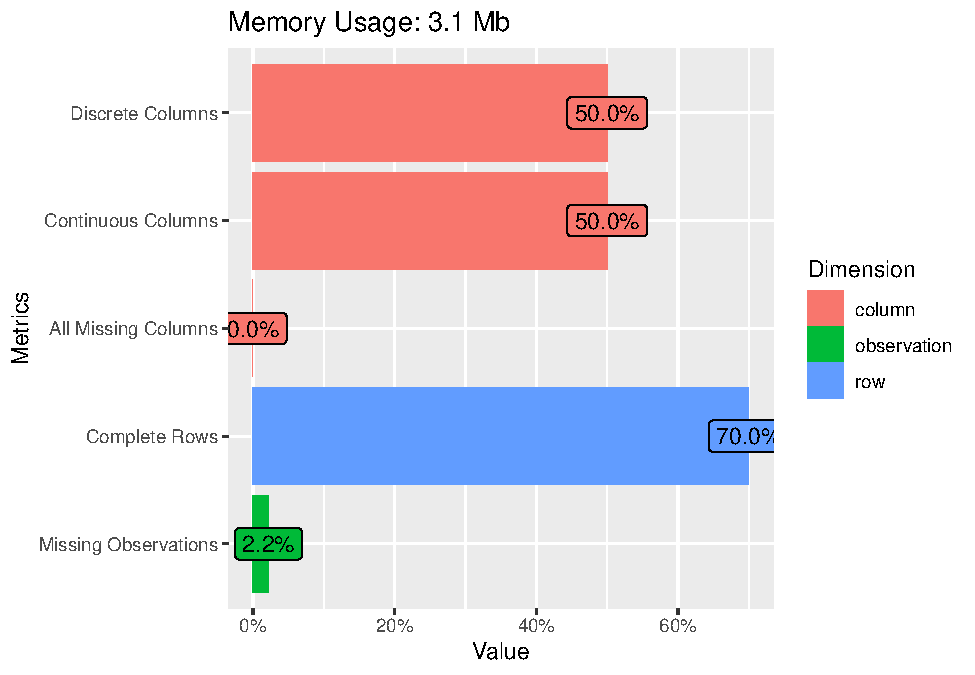
\includegraphics{_main_files/figure-latex/unnamed-chunk-4-1.pdf}

\begin{Shaded}
\begin{Highlighting}[]
\CommentTok{\#plots percentages missing across variables}
\FunctionTok{plot\_missing}\NormalTok{(data\_nba)}
\end{Highlighting}
\end{Shaded}

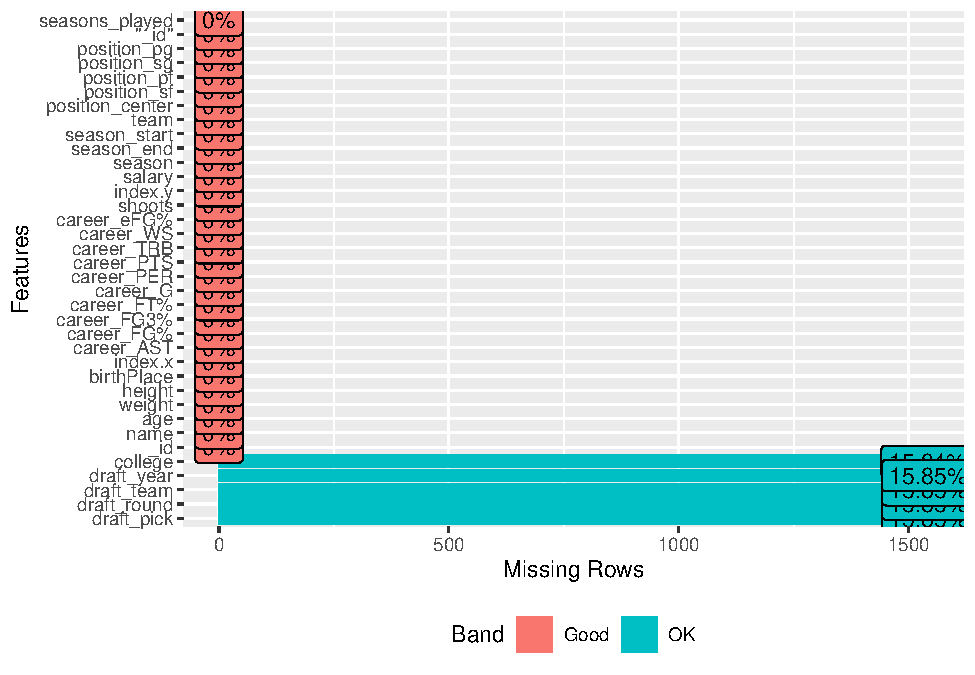
\includegraphics{_main_files/figure-latex/unnamed-chunk-4-2.pdf}

\begin{Shaded}
\begin{Highlighting}[]
\CommentTok{\# plots frequencies across variables}
\FunctionTok{plot\_bar}\NormalTok{(data\_nba)}
\end{Highlighting}
\end{Shaded}

\begin{verbatim}
## 11 columns ignored with more than 50 categories.
## X_id: 1794 categories
## name: 1790 categories
## birthPlace: 849 categories
## career_FG.: 333 categories
## career_FG3.: 297 categories
## career_FT.: 413 categories
## career_PER: 274 categories
## career_TRB: 113 categories
## career_eFG.: 310 categories
## college: 380 categories
## draft_pick: 67 categories
\end{verbatim}

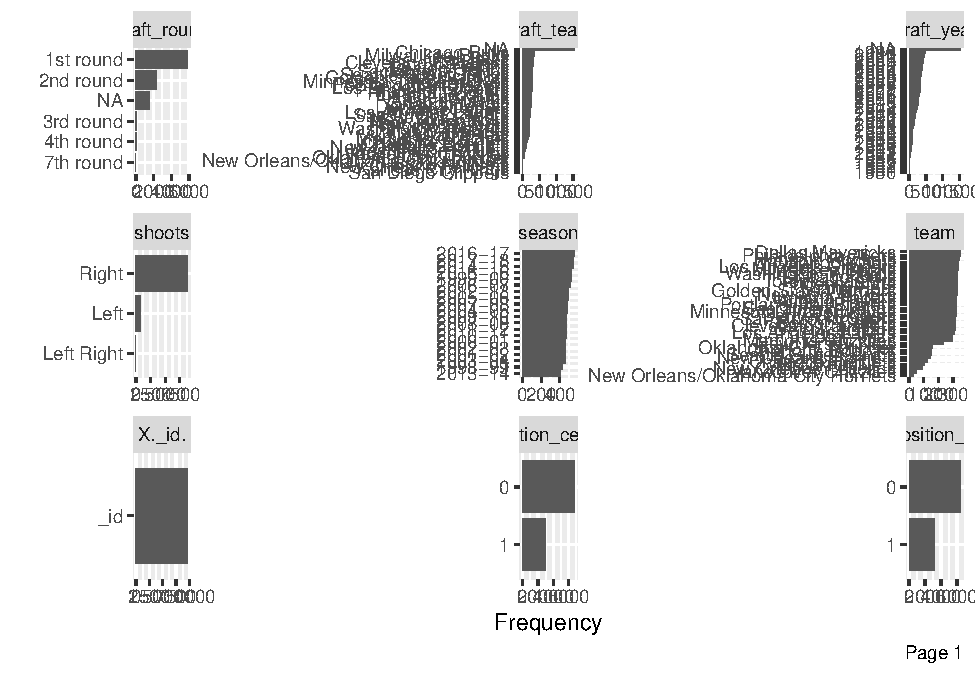
\includegraphics{_main_files/figure-latex/unnamed-chunk-4-3.pdf} 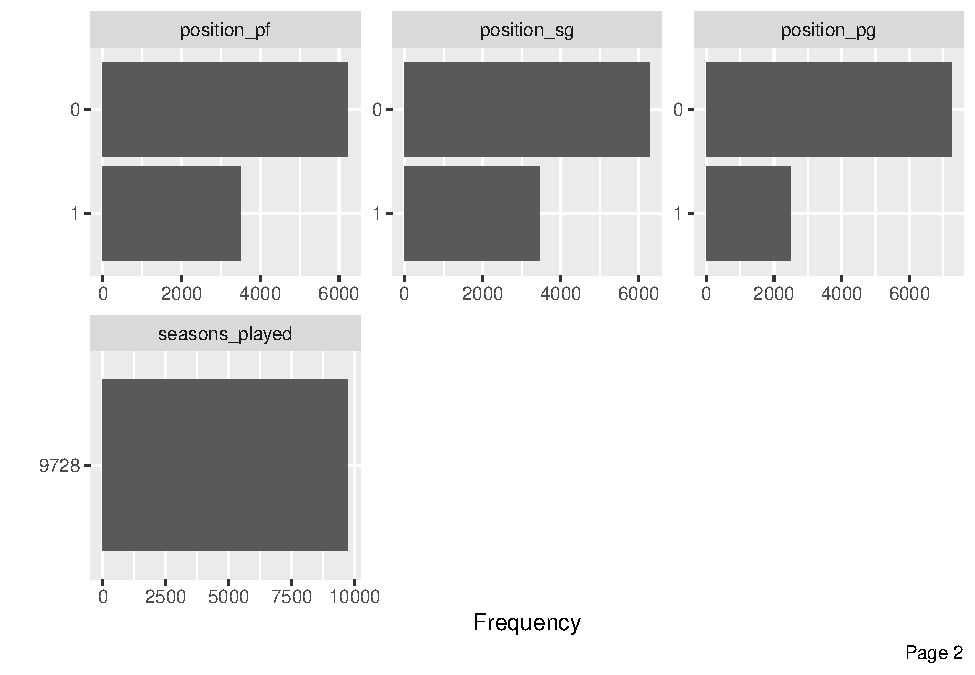
\includegraphics{_main_files/figure-latex/unnamed-chunk-4-4.pdf}

Now, let's try gtSummary for summary tables. A summary table is always a useful start once you have identified the type of varibales you are interested in.

Let's assume we are interested in age, seasons played, career ppints, salary,
position, and right or left handed (i.e.~``shoots'')

\begin{Shaded}
\begin{Highlighting}[]
\FunctionTok{library}\NormalTok{(gtsummary)}

\NormalTok{data\_nba }\SpecialCharTok{\%\textgreater{}\%} 
  \FunctionTok{select}\NormalTok{(age, seasons\_played, shoots, career\_PTS, salary, }\FunctionTok{contains}\NormalTok{(}\StringTok{"position"}\NormalTok{)) }\SpecialCharTok{\%\textgreater{}\%}
         \FunctionTok{tbl\_summary}\NormalTok{(}
           \AttributeTok{statistic =} \FunctionTok{all\_continuous}\NormalTok{() }\SpecialCharTok{\textasciitilde{}} \FunctionTok{c}\NormalTok{(}\StringTok{"\{mean\} (\{min\}, \{max\})"}\NormalTok{))}
\end{Highlighting}
\end{Shaded}

\begin{verbatim}
## Table printed with `knitr::kable()`, not {gt}. Learn why at
## https://www.danieldsjoberg.com/gtsummary/articles/rmarkdown.html
## To suppress this message, include `message = FALSE` in code chunk header.
\end{verbatim}

\begin{tabular}{l|c}
\hline
**Characteristic** & **N = 9,728**\\
\hline
age & 27.0 (18.0, 42.0)\\
\hline
seasons\_played & \\
\hline
9728 & 9,728 (100\%)\\
\hline
shoots & \\
\hline
Left & 856 (8.8\%)\\
\hline
Left Right & 7 (<0.1\%)\\
\hline
Right & 8,865 (91\%)\\
\hline
career\_PTS & 8.9 (0.0, 30.1)\\
\hline
salary & 4,072,633 (2,706, 34,682,550)\\
\hline
position\_center & 2,986 (31\%)\\
\hline
position\_sf & 3,222 (33\%)\\
\hline
position\_pf & 3,501 (36\%)\\
\hline
position\_sg & 3,447 (35\%)\\
\hline
position\_pg & 2,489 (26\%)\\
\hline
\end{tabular}

Now, let's look at a correlation matrix between all numeric
variables in the dataset.

\begin{Shaded}
\begin{Highlighting}[]
\FunctionTok{library}\NormalTok{(}\StringTok{"corrr"}\NormalTok{)}
\FunctionTok{library}\NormalTok{(}\StringTok{"corrplot"}\NormalTok{)}

\NormalTok{data\_nba\_numeric }\OtherTok{\textless{}{-}}\NormalTok{ data\_nba }\SpecialCharTok{\%\textgreater{}\%}
  \FunctionTok{select}\NormalTok{(}\FunctionTok{where}\NormalTok{(is.numeric)) }\SpecialCharTok{\%\textgreater{}\%}
  \FunctionTok{na.omit}\NormalTok{()}

\CommentTok{\# Find constant columns}
\NormalTok{constant\_columns }\OtherTok{\textless{}{-}} \FunctionTok{sapply}\NormalTok{(data\_nba\_numeric, }\ControlFlowTok{function}\NormalTok{(x) }\FunctionTok{length}\NormalTok{(}\FunctionTok{unique}\NormalTok{(x)) }\SpecialCharTok{==} \DecValTok{1}\NormalTok{)}

\CommentTok{\# Remove constant columns}
\NormalTok{data\_nba\_numeric }\OtherTok{\textless{}{-}}\NormalTok{ data\_nba\_numeric[, }\SpecialCharTok{!}\NormalTok{constant\_columns]}
\CommentTok{\# as number}
\NormalTok{corrmatrix }\OtherTok{\textless{}{-}}\NormalTok{ data\_nba\_numeric }\SpecialCharTok{\%\textgreater{}\%}
  \FunctionTok{correlate}\NormalTok{() }\SpecialCharTok{\%\textgreater{}\%}    \CommentTok{\# Create correlation data frame (cor\_df)}
  \FunctionTok{rearrange}\NormalTok{() }\SpecialCharTok{\%\textgreater{}\%}  \CommentTok{\# rearrange by correlations}
  \FunctionTok{shave}\NormalTok{() }

\FunctionTok{fashion}\NormalTok{(corrmatrix)}
\end{Highlighting}
\end{Shaded}

\begin{verbatim}
##               term career_AST position_pg career_PTS career_G career_WS
## 1       career_AST                                                     
## 2      position_pg        .61                                          
## 3       career_PTS        .61         .08                              
## 4         career_G        .47         .04        .65                   
## 5        career_WS        .52        -.01        .76      .83          
## 6      position_sg        .19         .22        .12      .09       .01
## 7           salary        .35        -.04        .60      .48       .59
## 8              age        .18         .03        .18      .49       .36
## 9      position_sf       -.08        -.33        .12      .13       .07
## 10      season_end        .01         .01        .04     -.17      -.09
## 11    season_start        .01         .01        .04     -.17      -.09
## 12         index.y        .01         .00       -.01     -.04      -.03
## 13         index.x        .01         .00       -.01     -.04      -.03
## 14          height       -.31        -.46       -.01     -.02      -.00
## 15     position_pf       -.29        -.44        .01      .11       .12
## 16 position_center       -.36        -.39       -.10      .04       .08
## 17          weight       -.49        -.66       -.06     -.03       .05
##    position_sg salary  age position_sf season_end season_start index.y index.x
## 1                                                                             
## 2                                                                             
## 3                                                                             
## 4                                                                             
## 5                                                                             
## 6                                                                             
## 7         -.03                                                                
## 8          .03    .25                                                         
## 9          .18    .03  .03                                                    
## 10         .02    .16 -.07        -.04                                        
## 11         .02    .16 -.07        -.04       1.00                             
## 12        -.05   -.02 -.02         .01       -.03         -.03                
## 13        -.06   -.02 -.02         .01       -.03         -.03    1.00        
## 14        -.03    .03 -.04         .30        .02          .02     .05     .05
## 15        -.46    .09  .03         .04       -.00         -.00     .01     .01
## 16        -.49    .10  .04        -.37       -.06         -.06     .01     .02
## 17        -.43    .12 -.07        -.01        .04          .04     .04     .04
##    height position_pf position_center weight
## 1                                           
## 2                                           
## 3                                           
## 4                                           
## 5                                           
## 6                                           
## 7                                           
## 8                                           
## 9                                           
## 10                                          
## 11                                          
## 12                                          
## 13                                          
## 14                                          
## 15    .15                                   
## 16    .12         .33                       
## 17    .41         .45             .66
\end{verbatim}

\begin{Shaded}
\begin{Highlighting}[]
\CommentTok{\# as plot}
\FunctionTok{rplot}\NormalTok{(corrmatrix)}
\end{Highlighting}
\end{Shaded}

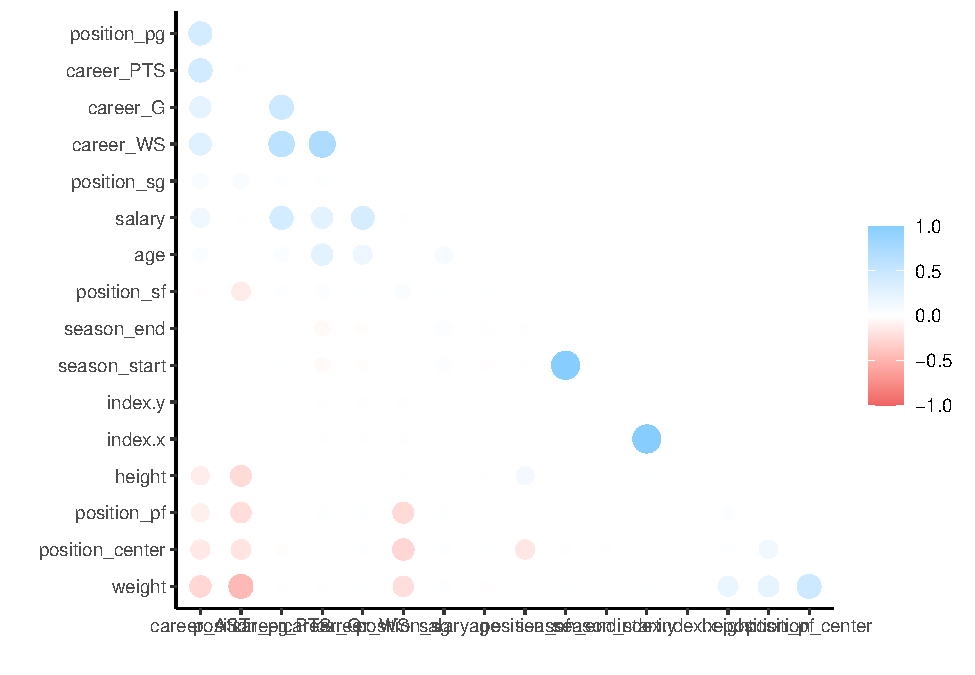
\includegraphics{_main_files/figure-latex/unnamed-chunk-6-1.pdf}

\begin{Shaded}
\begin{Highlighting}[]
\CommentTok{\# or...ggplot approach}
\FunctionTok{library}\NormalTok{(}\StringTok{"ggcorrplot"}\NormalTok{)}

\NormalTok{corrmatrix }\OtherTok{\textless{}{-}} \FunctionTok{round}\NormalTok{(}\FunctionTok{cor}\NormalTok{(data\_nba\_numeric), }\DecValTok{1}\NormalTok{)}

\FunctionTok{ggcorrplot}\NormalTok{(corrmatrix,}
           \AttributeTok{method =} \StringTok{"circle"}\NormalTok{,}
           \AttributeTok{type=}\StringTok{"lower"}\NormalTok{)}
\end{Highlighting}
\end{Shaded}

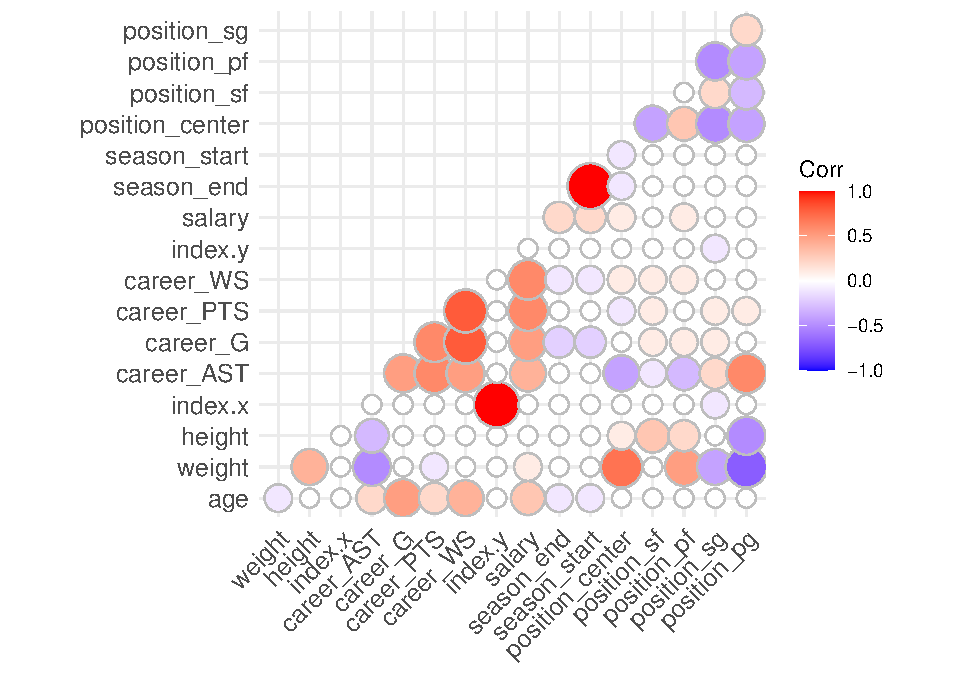
\includegraphics{_main_files/figure-latex/unnamed-chunk-6-2.pdf}

This is interesting for a first look. For example, it seems that the weight is
strongly correlated with whatever position you play. Centers are heavy, point
guards are light weights.
We also see that most performance metrics (``career\_\ldots{}'') are correlated with each
other and also with salary. Good players seem to be good in many things, and
good players seem to be paid more.

\hypertarget{explore-individual-variables}{%
\section{explore individual variables}\label{explore-individual-variables}}

Now, that we have a feeling for the whole dataset, we want to explore individual
variables. To keep it focused, we want to further explore the question
of whether players that score more on average are also paid more.

Maybe roles are clearly divided on the team. Maybe really good passers are highly
paid because they give great passes to people who then score. Or maybe teams
don't care about passers and just pay more to people who score more.

So, now, let's look at salary and average number of points scored by game.
Also, we want to know whether point guards (short people who pass a lot) are
paid less then other positions (who score more).

First, let's look how the two continuous variables are distributed:

\begin{Shaded}
\begin{Highlighting}[]
\NormalTok{data\_nba }\SpecialCharTok{\%\textgreater{}\%} \FunctionTok{ggplot}\NormalTok{() }\SpecialCharTok{+} 
\FunctionTok{geom\_boxplot}\NormalTok{(}\FunctionTok{aes}\NormalTok{(}\AttributeTok{y=}\NormalTok{salary)) }\SpecialCharTok{+}
  \FunctionTok{facet\_wrap}\NormalTok{(}\SpecialCharTok{\textasciitilde{}}\NormalTok{position\_pg) }\SpecialCharTok{+}
  \FunctionTok{theme\_light}\NormalTok{()}
\end{Highlighting}
\end{Shaded}

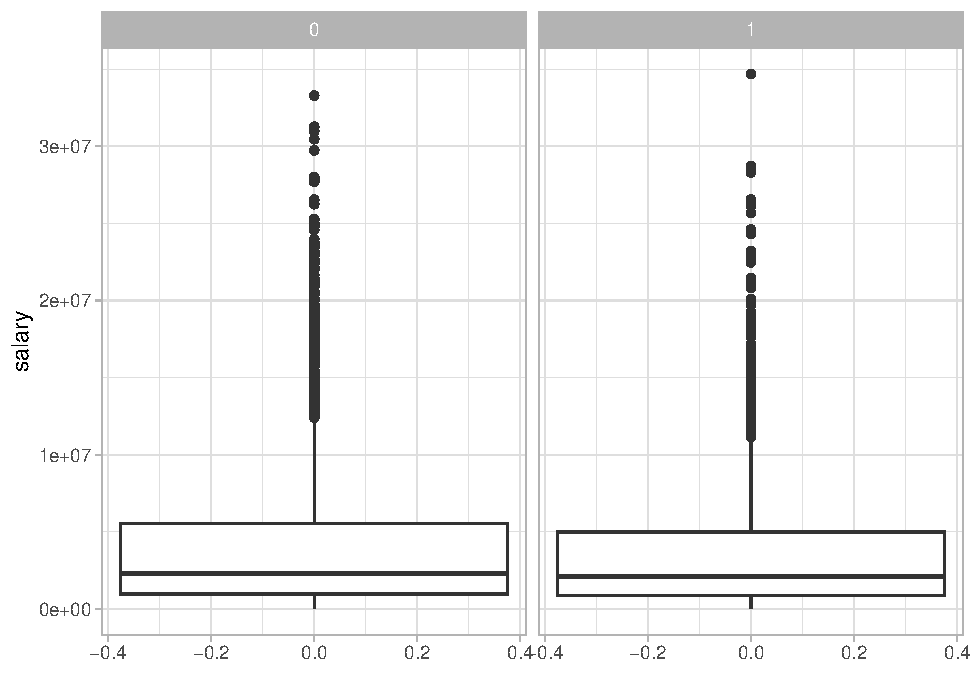
\includegraphics{_main_files/figure-latex/unnamed-chunk-7-1.pdf}

\begin{Shaded}
\begin{Highlighting}[]
\NormalTok{data\_nba }\SpecialCharTok{\%\textgreater{}\%} \FunctionTok{ggplot}\NormalTok{() }\SpecialCharTok{+} 
\FunctionTok{geom\_boxplot}\NormalTok{(}\FunctionTok{aes}\NormalTok{(}\AttributeTok{y=}\NormalTok{career\_PTS)) }\SpecialCharTok{+} 
  \FunctionTok{theme\_light}\NormalTok{()}
\end{Highlighting}
\end{Shaded}

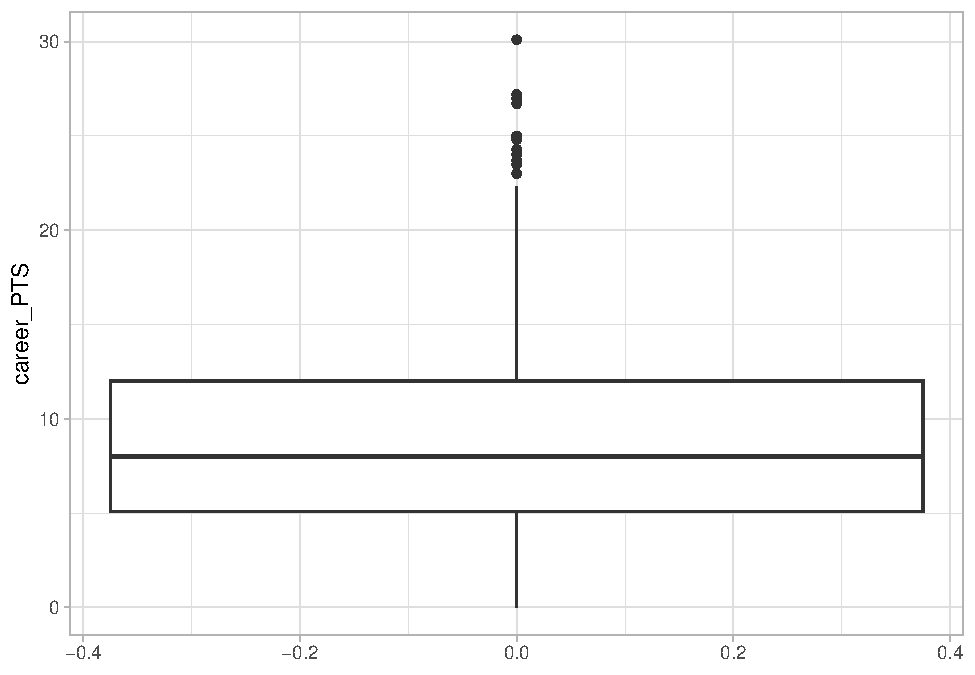
\includegraphics{_main_files/figure-latex/unnamed-chunk-7-2.pdf}

\begin{Shaded}
\begin{Highlighting}[]
\NormalTok{data\_nba }\SpecialCharTok{\%\textgreater{}\%} \FunctionTok{ggplot}\NormalTok{() }\SpecialCharTok{+} 
\FunctionTok{geom\_boxplot}\NormalTok{(}\FunctionTok{aes}\NormalTok{(}\AttributeTok{y=}\NormalTok{career\_PTS)) }\SpecialCharTok{+}
  \FunctionTok{facet\_wrap}\NormalTok{(}\SpecialCharTok{\textasciitilde{}}\NormalTok{position\_pg) }\SpecialCharTok{+}
  \FunctionTok{theme\_light}\NormalTok{()}
\end{Highlighting}
\end{Shaded}

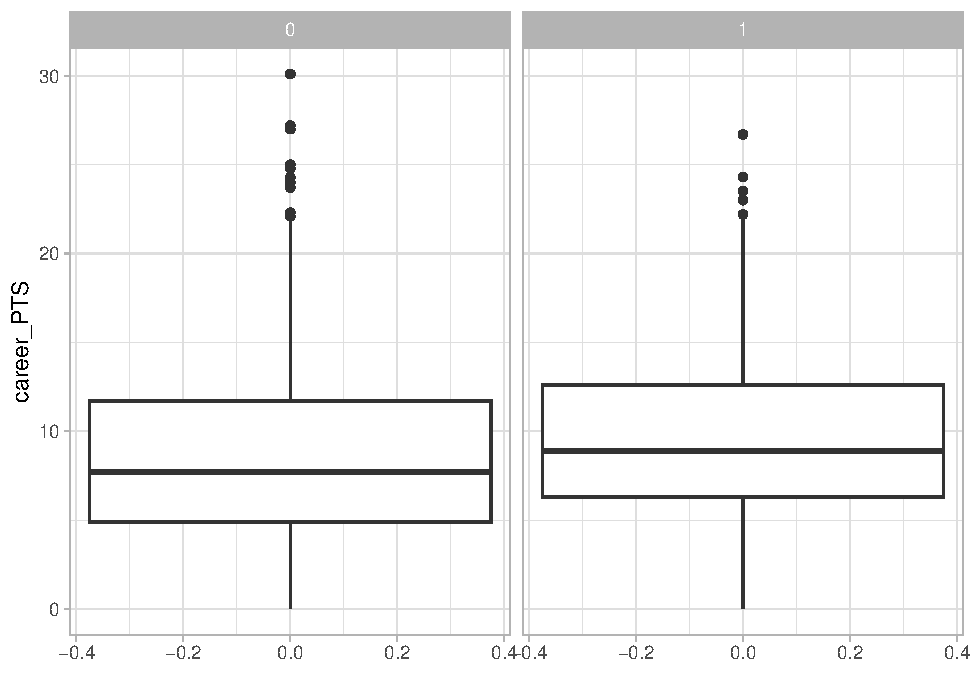
\includegraphics{_main_files/figure-latex/unnamed-chunk-7-3.pdf}

Let's look at the relationship between salary and position as well as the
relationship between position and points.

\begin{Shaded}
\begin{Highlighting}[]
\FunctionTok{str}\NormalTok{(data\_nba}\SpecialCharTok{$}\NormalTok{position\_pg)}
\end{Highlighting}
\end{Shaded}

\begin{verbatim}
##  num [1:9728] 1 0 0 0 0 0 0 0 0 0 ...
\end{verbatim}

\begin{Shaded}
\begin{Highlighting}[]
\FunctionTok{str}\NormalTok{(data\_nba}\SpecialCharTok{$}\NormalTok{salary)}
\end{Highlighting}
\end{Shaded}

\begin{verbatim}
##  num [1:9728] 798500 1411000 1594920 4500000 5062500 ...
\end{verbatim}

\begin{Shaded}
\begin{Highlighting}[]
\FunctionTok{str}\NormalTok{(data\_nba}\SpecialCharTok{$}\NormalTok{career\_pts)}
\end{Highlighting}
\end{Shaded}

\begin{verbatim}
## Warning: Unknown or uninitialised column: `career_pts`.
\end{verbatim}

\begin{verbatim}
##  NULL
\end{verbatim}

\begin{Shaded}
\begin{Highlighting}[]
\NormalTok{data\_nba }\SpecialCharTok{\%\textgreater{}\%} 
  \FunctionTok{ggplot}\NormalTok{() }\SpecialCharTok{+}
  \FunctionTok{geom\_bar}\NormalTok{(}\FunctionTok{aes}\NormalTok{(}\AttributeTok{x =}\NormalTok{ position\_pg, }
               \AttributeTok{y =}\NormalTok{ salary),}
           \AttributeTok{position =} \StringTok{"dodge"}\NormalTok{,}
           \AttributeTok{stat =} \StringTok{"summary"}\NormalTok{,}
           \AttributeTok{fun =} \StringTok{"mean"}\NormalTok{) }\SpecialCharTok{+} 
  \CommentTok{\#xlim(0, 10000000) +}
  \FunctionTok{labs}\NormalTok{(}\AttributeTok{title =} \StringTok{"Average salary (Point guard vs other positions)"}\NormalTok{,}
       \AttributeTok{subtitle =} \StringTok{"this is not that interesting"}\NormalTok{,}
       \AttributeTok{caption =} \StringTok{"Authors\textquotesingle{} calculation; NBA data 1998{-}2018"}\NormalTok{) }\SpecialCharTok{+}
  \FunctionTok{xlab}\NormalTok{(}\StringTok{"Player\textquotesingle{}s position"}\NormalTok{) }\SpecialCharTok{+}
  \FunctionTok{ylab}\NormalTok{(}\StringTok{"Player\textquotesingle{}s salary"}\NormalTok{) }\SpecialCharTok{+}
  \FunctionTok{theme\_minimal}\NormalTok{()}
\end{Highlighting}
\end{Shaded}

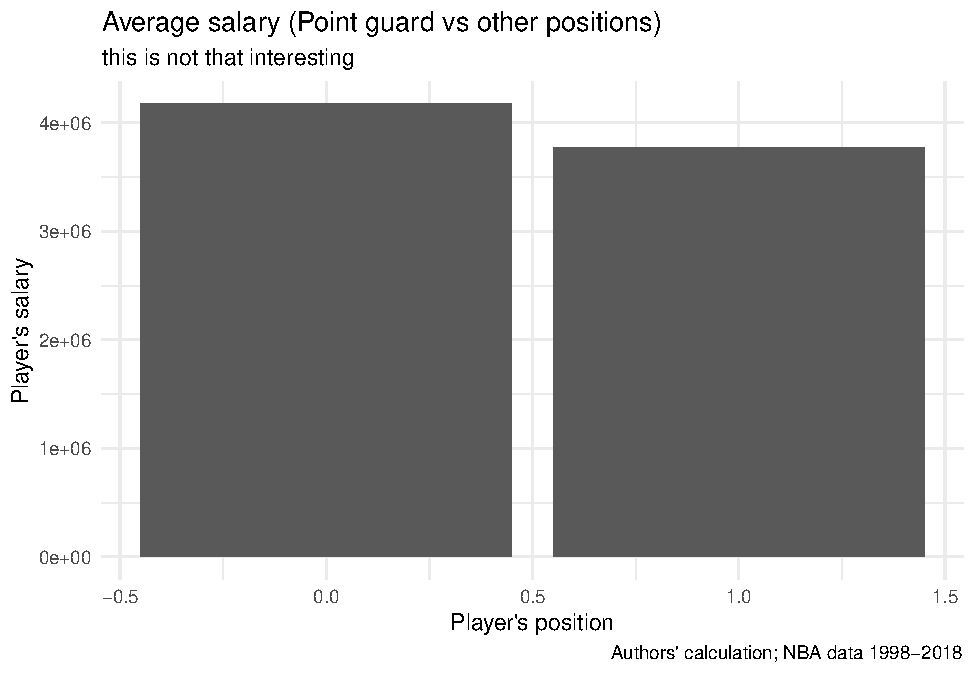
\includegraphics{_main_files/figure-latex/unnamed-chunk-8-1.pdf}

\begin{Shaded}
\begin{Highlighting}[]
\DocumentationTok{\#\# alternatively:}

\NormalTok{data\_nba }\SpecialCharTok{\%\textgreater{}\%} 
  \FunctionTok{group\_by}\NormalTok{(position\_pg) }\SpecialCharTok{\%\textgreater{}\%}
  \FunctionTok{summarize}\NormalTok{(}\AttributeTok{mean\_salary =} \FunctionTok{mean}\NormalTok{(salary, }\AttributeTok{na.rm=}\NormalTok{T)) }\SpecialCharTok{\%\textgreater{}\%}
  \FunctionTok{ggplot}\NormalTok{() }\SpecialCharTok{+}
  \FunctionTok{geom\_bar}\NormalTok{(}\FunctionTok{aes}\NormalTok{(}\AttributeTok{x =} \FunctionTok{as.factor}\NormalTok{(position\_pg), }
               \AttributeTok{y =}\NormalTok{ mean\_salary),}
           \AttributeTok{stat =} \StringTok{"identity"}\NormalTok{) }\SpecialCharTok{+} 
  \FunctionTok{ylim}\NormalTok{(}\DecValTok{0}\NormalTok{, }\DecValTok{6000000}\NormalTok{) }\SpecialCharTok{+}
  \FunctionTok{labs}\NormalTok{(}\AttributeTok{title =} \StringTok{"Average salary (Point guard vs other positions)"}\NormalTok{,}
       \AttributeTok{subtitle =} \StringTok{"this is not that interesting"}\NormalTok{,}
       \AttributeTok{caption =} \StringTok{"Authors\textquotesingle{} calculation; NBA data 1998{-}2018"}\NormalTok{) }\SpecialCharTok{+}
  \FunctionTok{xlab}\NormalTok{(}\StringTok{"Player\textquotesingle{}s position"}\NormalTok{) }\SpecialCharTok{+}
  \FunctionTok{ylab}\NormalTok{(}\StringTok{"Player\textquotesingle{}s salary (in million USD)"}\NormalTok{) }\SpecialCharTok{+}
  \FunctionTok{theme\_minimal}\NormalTok{()}
\end{Highlighting}
\end{Shaded}

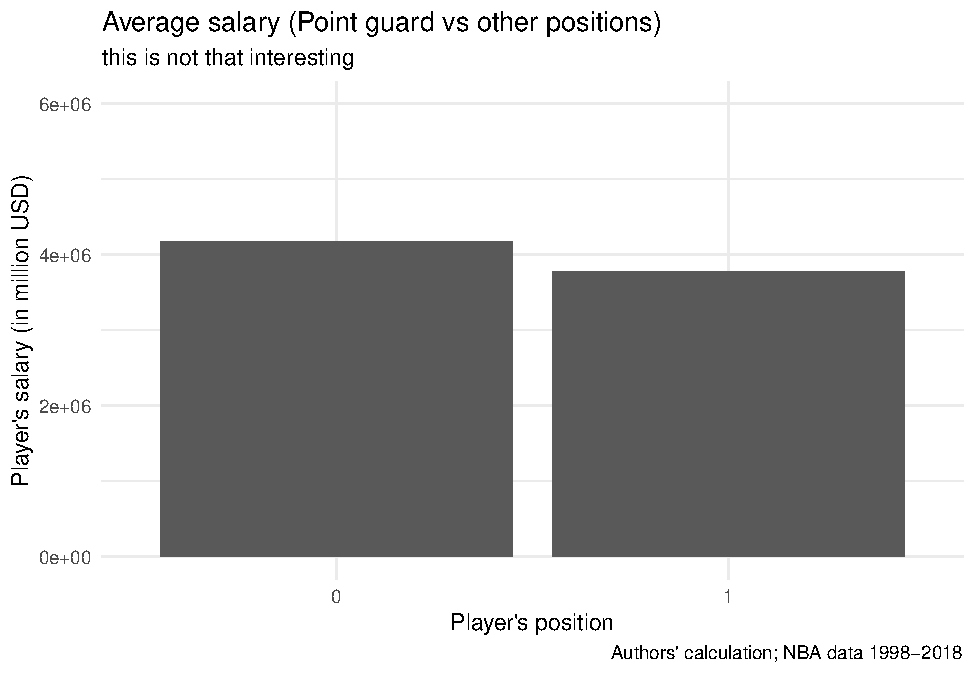
\includegraphics{_main_files/figure-latex/unnamed-chunk-8-2.pdf}

\begin{Shaded}
\begin{Highlighting}[]
\CommentTok{\# Now the relationship between position and points:}

\NormalTok{data\_nba }\SpecialCharTok{\%\textgreater{}\%} 
  \FunctionTok{group\_by}\NormalTok{(position\_pg) }\SpecialCharTok{\%\textgreater{}\%}
  \FunctionTok{summarize}\NormalTok{(}\AttributeTok{mean\_points =} \FunctionTok{mean}\NormalTok{(career\_PTS, }\AttributeTok{na.rm=}\NormalTok{T)) }\SpecialCharTok{\%\textgreater{}\%}
  \FunctionTok{ggplot}\NormalTok{() }\SpecialCharTok{+}
  \FunctionTok{geom\_bar}\NormalTok{(}\FunctionTok{aes}\NormalTok{(}\AttributeTok{x =} \FunctionTok{as.factor}\NormalTok{(position\_pg), }
               \AttributeTok{y =}\NormalTok{ mean\_points),}
           \AttributeTok{stat =} \StringTok{"identity"}\NormalTok{) }\SpecialCharTok{+} 
  \FunctionTok{ylim}\NormalTok{(}\DecValTok{0}\NormalTok{,}\DecValTok{15}\NormalTok{) }\SpecialCharTok{+}
  \FunctionTok{labs}\NormalTok{(}\AttributeTok{title =} \StringTok{"Average points per game (Point guard vs other positions)"}\NormalTok{,}
       \AttributeTok{subtitle =} \StringTok{"this is not that interesting"}\NormalTok{,}
       \AttributeTok{caption =} \StringTok{"Authors\textquotesingle{} calculation; NBA data 1998{-}2018"}\NormalTok{) }\SpecialCharTok{+}
  \FunctionTok{xlab}\NormalTok{(}\StringTok{"Player\textquotesingle{}s position"}\NormalTok{) }\SpecialCharTok{+}
  \FunctionTok{ylab}\NormalTok{(}\StringTok{"Points per game"}\NormalTok{) }\SpecialCharTok{+}
  \FunctionTok{theme\_minimal}\NormalTok{()}
\end{Highlighting}
\end{Shaded}

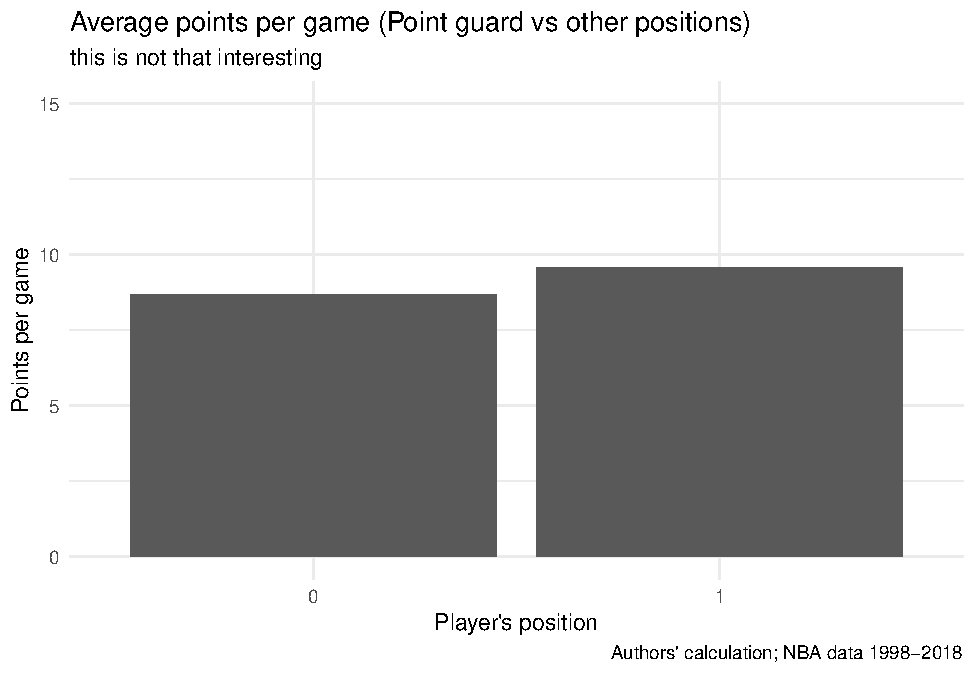
\includegraphics{_main_files/figure-latex/unnamed-chunk-8-3.pdf}

So, it seems that point gards are paid a little less even though they make a few more points on average. Interesting puzzle to explore.

\begin{Shaded}
\begin{Highlighting}[]
\CommentTok{\# find example for using histogramm()}
\CommentTok{\# find example for first just creating cross tabs as perecntages tbl\_cross(); summarize(); tabyl()}
\end{Highlighting}
\end{Shaded}

Now, let's explore the relationship which is at the heart of our analysis from now on: salary and average points.

\begin{Shaded}
\begin{Highlighting}[]
\CommentTok{\# simple scatterplot}
\NormalTok{data\_nba }\SpecialCharTok{\%\textgreater{}\%} \FunctionTok{ggplot}\NormalTok{() }\SpecialCharTok{+}
\FunctionTok{geom\_point}\NormalTok{(}\FunctionTok{aes}\NormalTok{(}\AttributeTok{y=}\NormalTok{salary, }\AttributeTok{x=}\NormalTok{career\_PTS)) }\SpecialCharTok{+} 
  \FunctionTok{theme\_minimal}\NormalTok{()}
\end{Highlighting}
\end{Shaded}

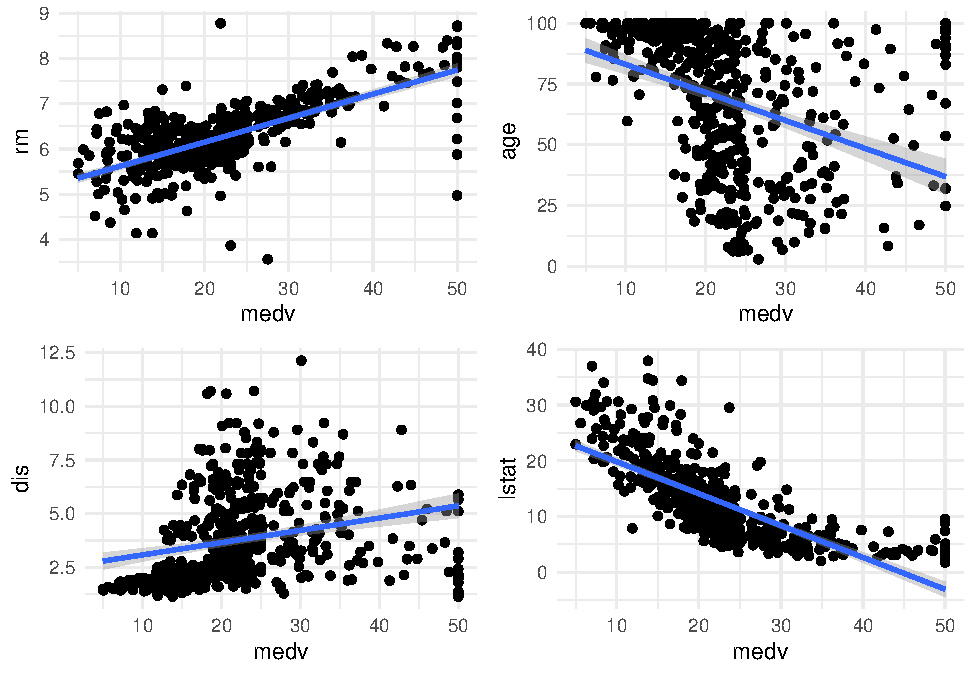
\includegraphics{_main_files/figure-latex/unnamed-chunk-10-1.pdf}

\begin{Shaded}
\begin{Highlighting}[]
\CommentTok{\# Now, let\textquotesingle{}s add a line}
\NormalTok{data\_nba }\SpecialCharTok{\%\textgreater{}\%} 
  \FunctionTok{ggplot}\NormalTok{(}\FunctionTok{aes}\NormalTok{(}\AttributeTok{y=}\NormalTok{salary, }\AttributeTok{x=}\NormalTok{career\_PTS)) }\SpecialCharTok{+}
    \FunctionTok{geom\_point}\NormalTok{() }\SpecialCharTok{+} 
     \FunctionTok{stat\_smooth}\NormalTok{(}\AttributeTok{method =} \StringTok{"lm"}\NormalTok{) }\SpecialCharTok{+} 
       \FunctionTok{theme\_minimal}\NormalTok{()}
\end{Highlighting}
\end{Shaded}

\begin{verbatim}
## `geom_smooth()` using formula = 'y ~ x'
\end{verbatim}

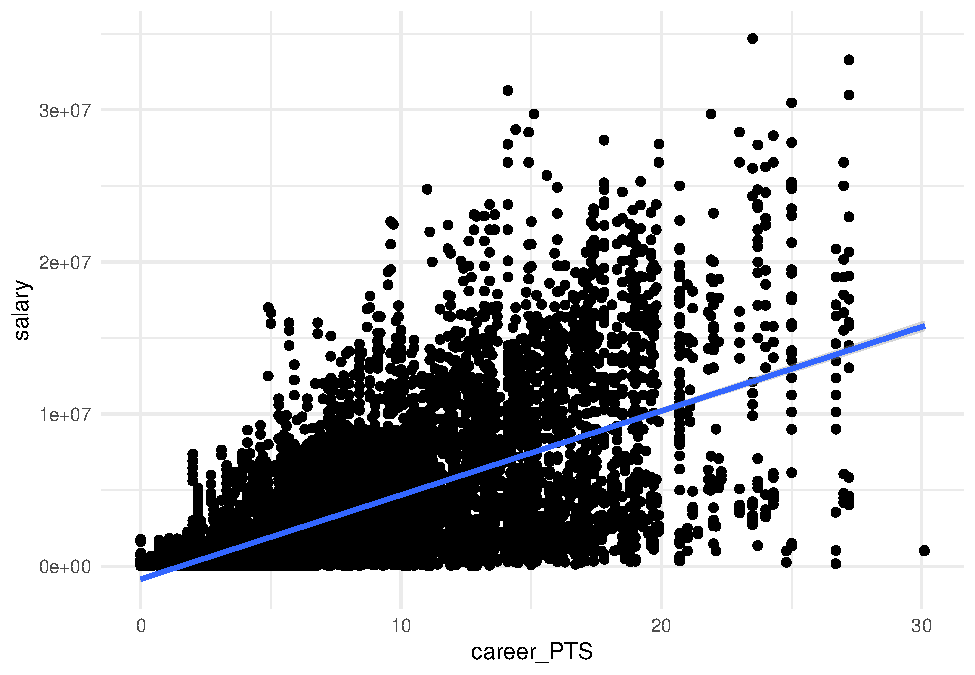
\includegraphics{_main_files/figure-latex/unnamed-chunk-10-2.pdf}

\begin{Shaded}
\begin{Highlighting}[]
\CommentTok{\# let\textquotesingle{}s look the relatiship separate for every year}
\NormalTok{data\_nba }\SpecialCharTok{\%\textgreater{}\%} 
  \FunctionTok{ggplot}\NormalTok{(}\FunctionTok{aes}\NormalTok{(}\AttributeTok{y=}\NormalTok{salary, }\AttributeTok{x=}\NormalTok{career\_PTS)) }\SpecialCharTok{+}
    \FunctionTok{geom\_point}\NormalTok{() }\SpecialCharTok{+} 
     \FunctionTok{stat\_smooth}\NormalTok{(}\AttributeTok{method =} \StringTok{"lm"}\NormalTok{) }\SpecialCharTok{+} 
        \FunctionTok{facet\_wrap}\NormalTok{(}\SpecialCharTok{\textasciitilde{}}\NormalTok{season\_start) }\SpecialCharTok{+} 
       \FunctionTok{theme\_minimal}\NormalTok{()}
\end{Highlighting}
\end{Shaded}

\begin{verbatim}
## `geom_smooth()` using formula = 'y ~ x'
\end{verbatim}

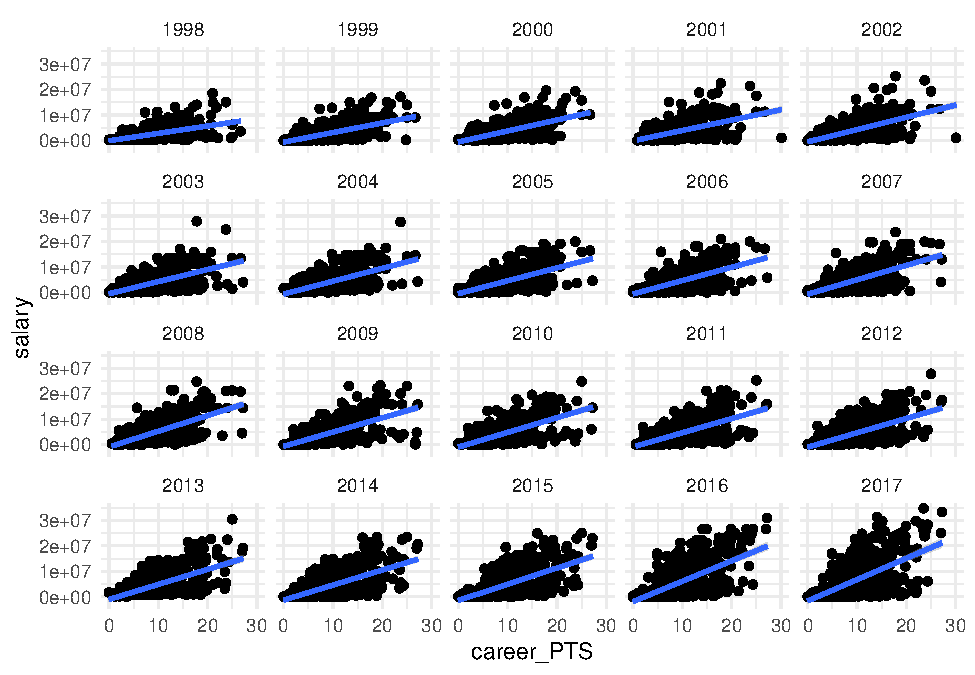
\includegraphics{_main_files/figure-latex/unnamed-chunk-10-3.pdf}

\begin{Shaded}
\begin{Highlighting}[]
\CommentTok{\# let\textquotesingle{}s look the relatiship for separate teams}
\NormalTok{data\_nba }\SpecialCharTok{\%\textgreater{}\%} 
  \FunctionTok{ggplot}\NormalTok{(}\FunctionTok{aes}\NormalTok{(}\AttributeTok{y=}\NormalTok{salary, }\AttributeTok{x=}\NormalTok{career\_PTS)) }\SpecialCharTok{+}
    \FunctionTok{geom\_point}\NormalTok{() }\SpecialCharTok{+} 
     \FunctionTok{stat\_smooth}\NormalTok{(}\AttributeTok{method =} \StringTok{"lm"}\NormalTok{) }\SpecialCharTok{+} 
        \FunctionTok{facet\_wrap}\NormalTok{(}\SpecialCharTok{\textasciitilde{}}\NormalTok{team) }\SpecialCharTok{+} 
       \FunctionTok{theme\_minimal}\NormalTok{()}
\end{Highlighting}
\end{Shaded}

\begin{verbatim}
## `geom_smooth()` using formula = 'y ~ x'
\end{verbatim}

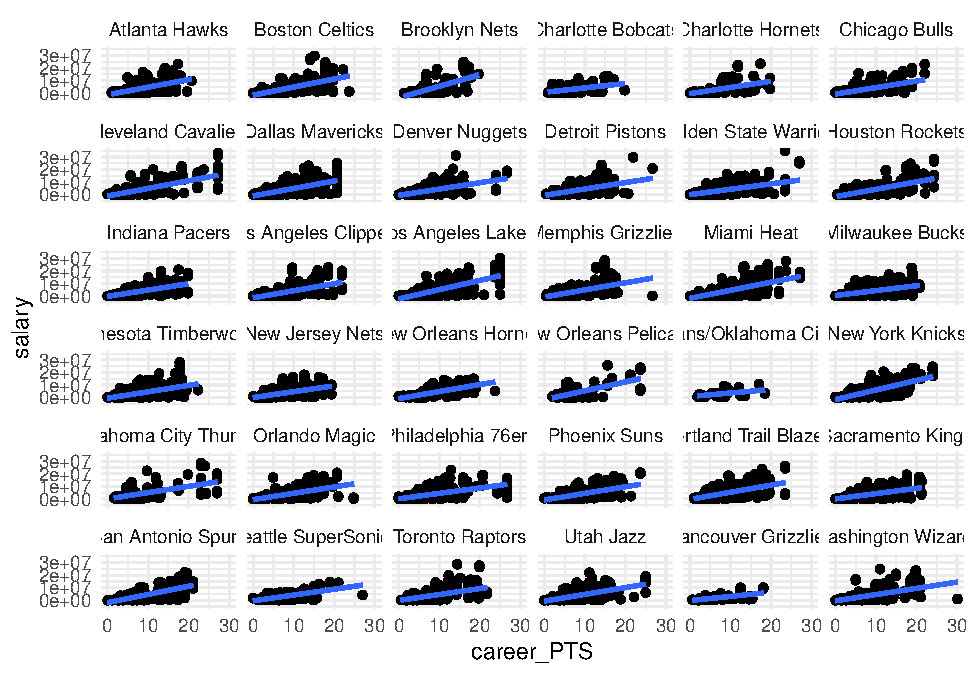
\includegraphics{_main_files/figure-latex/unnamed-chunk-10-4.pdf}

\begin{Shaded}
\begin{Highlighting}[]
\CommentTok{\# let\textquotesingle{}s look at it by position}
\NormalTok{scatter\_pg }\OtherTok{\textless{}{-}}\NormalTok{ data\_nba }\SpecialCharTok{\%\textgreater{}\%} \FunctionTok{filter}\NormalTok{(position\_pg }\SpecialCharTok{==}\DecValTok{1}\NormalTok{) }\SpecialCharTok{\%\textgreater{}\%}
  \FunctionTok{ggplot}\NormalTok{(}\FunctionTok{aes}\NormalTok{(}\AttributeTok{y=}\NormalTok{salary, }\AttributeTok{x=}\NormalTok{career\_PTS)) }\SpecialCharTok{+}
    \FunctionTok{geom\_point}\NormalTok{() }\SpecialCharTok{+} 
     \FunctionTok{stat\_smooth}\NormalTok{(}\AttributeTok{method =} \StringTok{"lm"}\NormalTok{) }\SpecialCharTok{+} 
       \FunctionTok{theme\_minimal}\NormalTok{()}

\NormalTok{scatter\_center }\OtherTok{\textless{}{-}}\NormalTok{ data\_nba }\SpecialCharTok{\%\textgreater{}\%} \FunctionTok{filter}\NormalTok{(position\_center }\SpecialCharTok{==}\DecValTok{1}\NormalTok{) }\SpecialCharTok{\%\textgreater{}\%}
  \FunctionTok{ggplot}\NormalTok{(}\FunctionTok{aes}\NormalTok{(}\AttributeTok{y=}\NormalTok{salary, }\AttributeTok{x=}\NormalTok{career\_PTS)) }\SpecialCharTok{+}
    \FunctionTok{geom\_point}\NormalTok{() }\SpecialCharTok{+} 
     \FunctionTok{stat\_smooth}\NormalTok{(}\AttributeTok{method =} \StringTok{"lm"}\NormalTok{) }\SpecialCharTok{+} 
       \FunctionTok{theme\_minimal}\NormalTok{()}

\NormalTok{scatter\_pf }\OtherTok{\textless{}{-}}\NormalTok{ data\_nba }\SpecialCharTok{\%\textgreater{}\%} \FunctionTok{filter}\NormalTok{(position\_pf }\SpecialCharTok{==}\DecValTok{1}\NormalTok{) }\SpecialCharTok{\%\textgreater{}\%}
  \FunctionTok{ggplot}\NormalTok{(}\FunctionTok{aes}\NormalTok{(}\AttributeTok{y=}\NormalTok{salary, }\AttributeTok{x=}\NormalTok{career\_PTS)) }\SpecialCharTok{+}
    \FunctionTok{geom\_point}\NormalTok{() }\SpecialCharTok{+} 
     \FunctionTok{stat\_smooth}\NormalTok{(}\AttributeTok{method =} \StringTok{"lm"}\NormalTok{) }\SpecialCharTok{+} 
       \FunctionTok{theme\_minimal}\NormalTok{()}

\NormalTok{scatter\_sf }\OtherTok{\textless{}{-}}\NormalTok{ data\_nba }\SpecialCharTok{\%\textgreater{}\%} \FunctionTok{filter}\NormalTok{(position\_sf }\SpecialCharTok{==}\DecValTok{1}\NormalTok{) }\SpecialCharTok{\%\textgreater{}\%}
  \FunctionTok{ggplot}\NormalTok{(}\FunctionTok{aes}\NormalTok{(}\AttributeTok{y=}\NormalTok{salary, }\AttributeTok{x=}\NormalTok{career\_PTS)) }\SpecialCharTok{+}
    \FunctionTok{geom\_point}\NormalTok{() }\SpecialCharTok{+} 
     \FunctionTok{stat\_smooth}\NormalTok{(}\AttributeTok{method =} \StringTok{"lm"}\NormalTok{) }\SpecialCharTok{+} 
       \FunctionTok{theme\_minimal}\NormalTok{()}

\FunctionTok{library}\NormalTok{(}\StringTok{"ggpubr"}\NormalTok{)}
\end{Highlighting}
\end{Shaded}

\begin{verbatim}
## Warning: package 'ggpubr' was built under R version 4.2.3
\end{verbatim}

\begin{Shaded}
\begin{Highlighting}[]
\FunctionTok{ggarrange}\NormalTok{(scatter\_center, scatter\_pf,}
\NormalTok{          scatter\_sf, scatter\_pg,}
          \AttributeTok{ncol =} \DecValTok{2}\NormalTok{, }\AttributeTok{nrow =} \DecValTok{2}\NormalTok{,}
          \AttributeTok{labels =} \FunctionTok{c}\NormalTok{(}\StringTok{"Center"}\NormalTok{,}
                     \StringTok{"Power Forward"}\NormalTok{,}
                     \StringTok{"Small Forward"}\NormalTok{,}
                     \StringTok{"Point Guard"}\NormalTok{))}
\end{Highlighting}
\end{Shaded}

\begin{verbatim}
## `geom_smooth()` using formula = 'y ~ x'
## `geom_smooth()` using formula = 'y ~ x'
## `geom_smooth()` using formula = 'y ~ x'
## `geom_smooth()` using formula = 'y ~ x'
\end{verbatim}

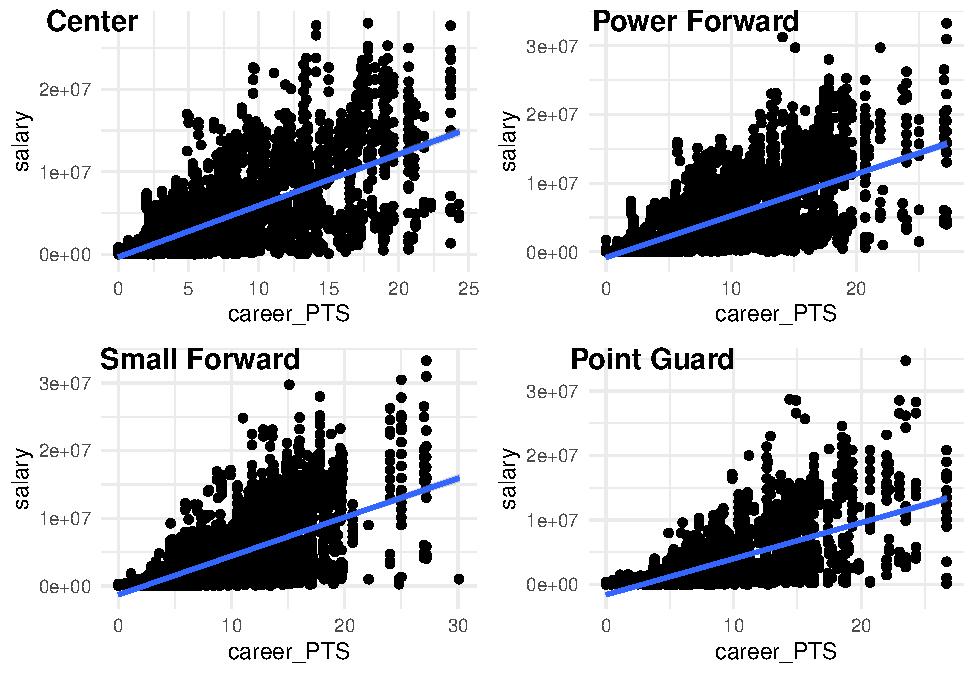
\includegraphics{_main_files/figure-latex/unnamed-chunk-10-5.pdf}

\begin{Shaded}
\begin{Highlighting}[]
\CommentTok{\# yet a better way to compare this could be:}

\NormalTok{data\_nba }\SpecialCharTok{\%\textgreater{}\%} 
  \FunctionTok{ggplot}\NormalTok{(}\FunctionTok{aes}\NormalTok{(}\AttributeTok{y=}\NormalTok{salary, }\AttributeTok{x=}\NormalTok{career\_PTS, }\AttributeTok{color=}\FunctionTok{as.factor}\NormalTok{(position\_pg))) }\SpecialCharTok{+}
    \FunctionTok{geom\_point}\NormalTok{() }\SpecialCharTok{+} 
     \FunctionTok{stat\_smooth}\NormalTok{(}\AttributeTok{method =} \StringTok{"lm"}\NormalTok{,}
                 \FunctionTok{aes}\NormalTok{(}\AttributeTok{group=}\FunctionTok{as.factor}\NormalTok{(position\_pg))) }\SpecialCharTok{+} 
       \FunctionTok{theme\_minimal}\NormalTok{()}
\end{Highlighting}
\end{Shaded}

\begin{verbatim}
## `geom_smooth()` using formula = 'y ~ x'
\end{verbatim}

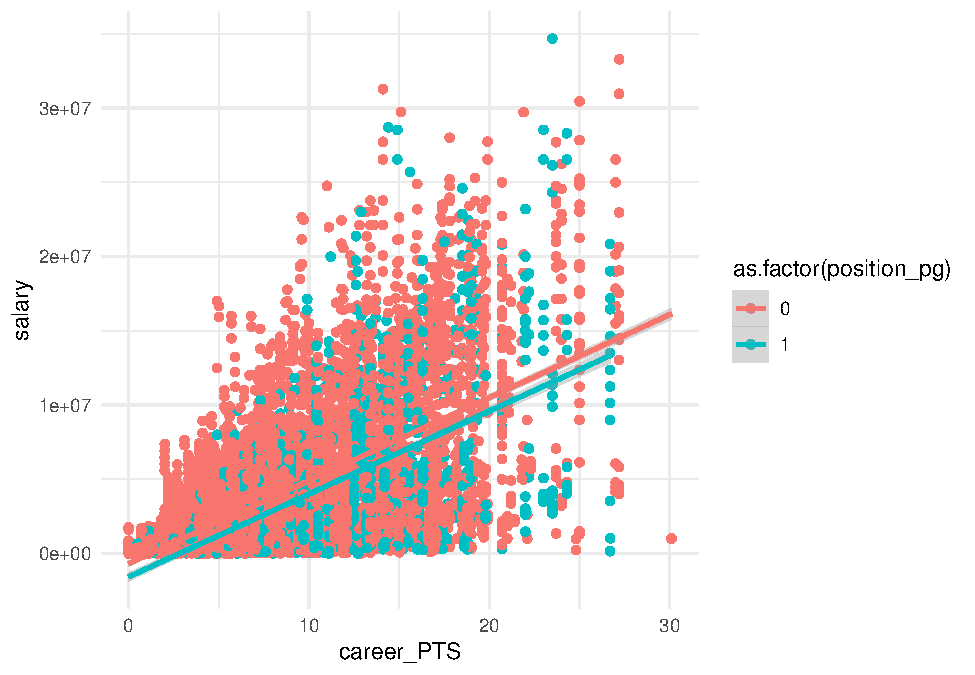
\includegraphics{_main_files/figure-latex/unnamed-chunk-10-6.pdf}

\begin{Shaded}
\begin{Highlighting}[]
\NormalTok{data\_nba }\SpecialCharTok{\%\textgreater{}\%} 
  \FunctionTok{ggplot}\NormalTok{(}\FunctionTok{aes}\NormalTok{(}\AttributeTok{y=}\NormalTok{salary, }\AttributeTok{x=}\NormalTok{career\_PTS, }\AttributeTok{color=}\FunctionTok{as.factor}\NormalTok{(position\_center))) }\SpecialCharTok{+}
    \FunctionTok{geom\_point}\NormalTok{() }\SpecialCharTok{+} 
     \FunctionTok{stat\_smooth}\NormalTok{(}\AttributeTok{method =} \StringTok{"lm"}\NormalTok{,}
                 \FunctionTok{aes}\NormalTok{(}\AttributeTok{group=}\FunctionTok{as.factor}\NormalTok{(position\_center))) }\SpecialCharTok{+} 
       \FunctionTok{theme\_minimal}\NormalTok{()}
\end{Highlighting}
\end{Shaded}

\begin{verbatim}
## `geom_smooth()` using formula = 'y ~ x'
\end{verbatim}

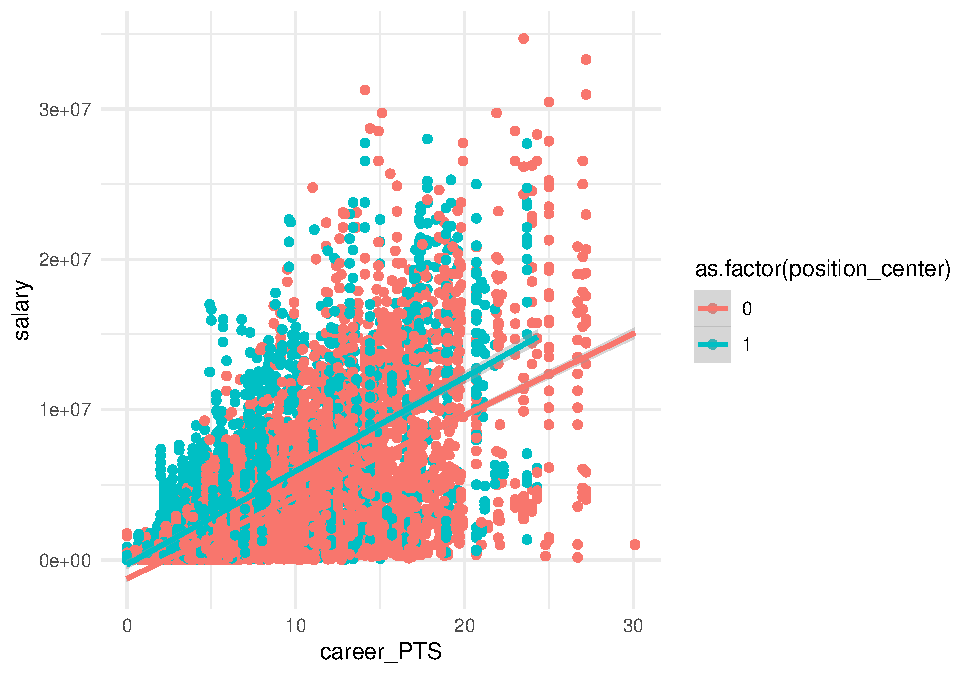
\includegraphics{_main_files/figure-latex/unnamed-chunk-10-7.pdf}

Let's reflect a moment what we can learn from all this.

First, there seems to be a somewhat linear relationship between how many points
a player scores and how much they are paid. This relationship seems pretty robust across years and teams. It also holds true for point guards just as much as for non-point guards. However, the average salary for point guards is lower in comparison. We also learn that the link between salary and points is stronger for centers. They seems to be paid more, the more they score.

We have set the stage now for linear regression (next week). Linear regression
is all about further exploring the relationship between two variables, one outcome (often called ``y'') and one independent variable (often called ``x''). Independent variables have many names. They are sometimes called ``covariates''; ``predictors''; ``exposure'', depending on the context.

There are a number of cool things that regression can do for us that simple EDA cannot:

\begin{enumerate}
\def\labelenumi{\arabic{enumi})}
\item
  It can model the relationship between two variables while considering simultaneously the potential influence of other factors. Image we are interested
  in the effect of points per game on salary regardless of position, season or team.
  With regression we can estimate how much more a player would ear every season
  if he scored 10 more points a game (regardless of the position he plays).
\item
  It can assess what explains the effect of one variable on another (i.e.~mediation). Maybe we find that point guards earn less and we want to know why. Is it because they score less? Is it because they play less time on average?
\item
  It can be used to predict salaries for players for whom we don't know the salary or even for hypothetical players. We could also look at the performance trend of players and predict whether they earn more next season or not.
\end{enumerate}

\hypertarget{eda-2}{%
\chapter{Exploratory Data Analysis - II}\label{eda-2}}

This week we will try to apply our last weeks knowledge into analysis.

\hypertarget{markdown-introduction}{%
\section{Markdown Introduction}\label{markdown-introduction}}

R Markdown is a powerful tool that allows you to create dynamic documents, presentations, and reports using R code. It combines the core syntax of markdown (an easy-to-write plain text format) with embedded R code chunks that are run when the document is rendered¹.

R Markdown documents are fully reproducible, meaning that anyone can re-run the code and generate the same results. This makes it easy to share your work with others and ensure that your results are accurate and reliable.

One of the great things about R Markdown is its flexibility. You can use it to create a wide variety of output formats, including HTML, PDF, and Microsoft Word documents. You can even create interactive documents with Shiny components¹.

To get started with R Markdown, you'll need to install the \texttt{rmarkdown} package from CRAN. This can be done by running the command \texttt{install.packages("rmarkdown")} in the R console². Once you have the package installed, you can create a new R Markdown document in RStudio by going to \texttt{File\ \textgreater{}\ New\ File\ \textgreater{}\ R\ Markdown}.

An R Markdown document is made up of text written in markdown syntax and chunks of R code. When you render the document, the R code is executed and its output (such as plots or tables) is inserted into the final document¹.

When you render this document, the text and code will be combined to create an HTML file that includes both the markdown text and the output of the R code chunks.

You can easily add images to an R Markdown document using the standard markdown syntax for images. The basic syntax for adding an image is \texttt{!{[}Alt\ text{]}(image\_url)}, where \texttt{Alt\ text} is the text that will be displayed if the image cannot be loaded, and \texttt{image\_url} is the URL of the image you want to include.

I hope this helps you understand how to add images to an R Markdown document! Let me know if you have any further questions 😊

R Markdown is a powerful tool that offers many advantages for data analysis and reporting. Some of the key benefits of using R Markdown include:

\begin{enumerate}
\def\labelenumi{\arabic{enumi}.}
\item
  \textbf{Reproducibility}: R Markdown documents are fully reproducible, meaning that anyone can re-run the code and generate the same results. This makes it easy to share your work with others and ensure that your results are accurate and reliable.
\item
  \textbf{Flexibility}: R Markdown is incredibly flexible and can be used to create a wide variety of output formats, including HTML, PDF, and Microsoft Word documents. You can even create interactive documents with Shiny components.
\item
  \textbf{Ease of use}: R Markdown is easy to use, even for people with little or no programming experience. The core syntax of markdown is simple and intuitive, and the ability to embed R code directly into the document makes it easy to include dynamic content.
\item
  \textbf{Integration with R}: R Markdown is tightly integrated with R, making it easy to access and use the full power of the R language for data analysis and visualization.
\item
  \textbf{Collaboration}: R Markdown makes it easy to collaborate with others on data analysis projects. You can share your code and results with others, and they can easily reproduce your work and build on it.
\end{enumerate}

Overall, R Markdown is a powerful tool that offers many advantages for data analysis and reporting. It's a great way to create dynamic, reproducible documents that are easy to share and collaborate on 😊

I hope this introduction helps you understand what R Markdown is and how it can be used. If you want to learn more, there are many great resources available online, including the \href{\%5E1\%5E}{R Markdown website} 😊

\hypertarget{applying-edawvsown-data}{%
\section{Applying EDA(WVS/own data)}\label{applying-edawvsown-data}}

\hypertarget{exercise---1}{%
\subsection{Exercise - 1}\label{exercise---1}}

\begin{enumerate}
\def\labelenumi{\arabic{enumi}.}
\item
  Write a script to load an R data file using the \texttt{load()} function. What does this function do and what is the format of the data file that it can read?
\item
  Use the \texttt{read\_excel()} function to read data from an Excel file. What arguments does this function take and what is the format of the data that it returns?
\item
  Use the \texttt{str()} and \texttt{glimpse()} functions to inspect the structure of a data frame. What is the difference between these two functions and when would you use one over the other?
\item
  Use the \texttt{table()} function to create a frequency table of a categorical variable in a data frame. How can you use this function to summarize data?
\item
  Use the \texttt{summary()} function to generate summary statistics for a numeric variable in a data frame. What statistics does this function return by default and how can you customize its output?
\item
  Use the \texttt{mutate()} function to create a new variable in a data frame based on existing variables. Provide an example of how you would use this function.
\item
  Use the \texttt{case\_when()} function to recode a categorical variable in a data frame based on certain conditions. Provide an example of how you would use this function.
\item
  Use the \texttt{ggplot()} function to create a scatter plot of two numeric variables in a data frame. What arguments does this function take and how can you customize the appearance of the plot?
\item
  Use the \texttt{corr()} function to calculate the correlation between two numeric variables in a data frame. What is correlation and how is it calculated?
\end{enumerate}

\textbf{This is a draft of questions, dataframe and the variables will be specified later}

\hypertarget{dags-1}{%
\chapter{DAGs}\label{dags-1}}

\begin{itemize}
\tightlist
\item
  Before Linear Regression
\item
  2 main reasons to model

  \begin{itemize}
  \tightlist
  \item
    understand causal effects -\textgreater{} DAGs
  \item
    predict -\textgreater{} later
  \end{itemize}
\end{itemize}

\hypertarget{causality}{%
\section{Causality}\label{causality}}

\begin{itemize}
\tightlist
\item
  Correlation does not equal Causation

  \begin{itemize}
  \tightlist
  \item
    Examples
  \end{itemize}
\item
  Identification of (causal) effect(s) of interest
\end{itemize}

\hypertarget{dags}{%
\section{DAGs}\label{dags}}

\begin{itemize}
\tightlist
\item
  Indirect causal effect/Overcontrol Bias/Pipe
\item
  Confounders/Fork
\item
  Colliders
\item
  Each with individual examples

  \begin{itemize}
  \tightlist
  \item
    Maybe one big example
  \end{itemize}
\end{itemize}

\hypertarget{totaldirect-effect}{%
\section{Total/Direct effect}\label{totaldirect-effect}}

\begin{itemize}
\tightlist
\item
  Identification
\end{itemize}

\hypertarget{dagitty.net}{%
\section{dagitty.net}\label{dagitty.net}}

\hypertarget{lin-t-1}{%
\chapter{Linear Regression Theory I: Simple Linear Regression}\label{lin-t-1}}

\hypertarget{what-is-linear-regression}{%
\section{What is Linear Regression}\label{what-is-linear-regression}}

When we use statistical modelling in social sciences there are two main
approaches.
The more classical approach is to use modelling for estimating the effect that
one or several independent variables have on one dependent variable. Maybe we
are interested in knowing if a higher income has an effect on life satisfaction
and if yes, what the direction and magnitude of this effect is. Does more money
actually make you happier?

The other and more recent approach is to use modelling for making predictions
with high accuracy. Based on the relationships between many independent
variables and one dependent variable, we try to predict the latter for actual
or hypothetical cases and their individual values for the independent variables.
This approach lies at the heart of \emph{machine learning} and drives many of the
technologies we use on a daily basis from E-Mail spam filters to ChatGPT.

Linear regression is one of the many available modelling techniques and it can
serve both approaches lined out above. In this session we will focus on using
linear regression for estimating an effect of interest but we will return to
prediction at a later point in this course.

But how do we know if we should choose linear regression for a specific task?
This is not easy to answer as there are many alternatives and even variations of
linear regression which may be better suited for a specific empirical problem.
As this is an introduction to modelling and time is of the essence we opted to
reduce the options and focus on two kind of models over the next weeks. Linear
regression and logistic regression. Both are comparably easy to understand and
use. Also, if we understand both of these techniques, we are in a good position
to build upon our knowledge and learn all of those more complex and specific
models that we will encounter in textbooks and scientific papers.

With the pool of options trimmed down to two, the question remains unanswered.
Should I use linear or logistic regression for my task? But now the answer is
relatively straightforward. What is the type of our dependent variable? Is it
metric? Then we use linear regression. Is it binary or categorical? Then we use
logistic regression. Linear regression will be the focus of this and the next
weeks and then we will turn to logistic regression.

Now let us dive in and learn what linear regression is all about.

\hypertarget{examplary-research-question-data}{%
\section{Examplary research question \& data}\label{examplary-research-question-data}}

Let us imagine that we are interested in a research question that asks what
makes a good grade in a seminar paper. In particular we are interested in the
effect that the hours a student invests in working on it has on the grade. Based
on some theoretical considerations, and maybe some idealistic views, we derive
our main hypotheses that putting in more hours will result in a better grade.

Now we also - hypothetically - held a small survey and asked 200 imaginary
students some questions on how they approached writing a seminar paper. In
particular we asked them how much time they spent working on the paper, if they
have attended (almost) all seminar sessions, how closely they worked with their
lecturers in preparing the paper and what the mean grade for previous papers
was. As these imaginary students have already turned in their papers, we also
know the grades they achieved.

Please note, that this is data on \textbf{imaginary} students, meaning we have
simulated the data making some assumptions on how to achieve a good (or bad)
grade in a paper. The assumptions we made do not necessarily reflect the way
\emph{you} write a good paper while still being based in our experience on what it
takes to achieve a good grade. But remember, no real students were harmed in
making up this example data.

Let us have a first look on the data:
XXX ALIGN WITH EDA XXX

\begin{verbatim}
## Warning: package 'skimr' was built under R version 4.2.3
\end{verbatim}

\begin{verbatim}
## 
## Attaching package: 'skimr'
\end{verbatim}

\begin{verbatim}
## The following object is masked from 'package:corrr':
## 
##     focus
\end{verbatim}

\begin{verbatim}
## Warning: package 'knitr' was built under R version 4.2.3
\end{verbatim}

\begin{tabular}{l|l|r|r|l|r|l|r|l|r|r|r|r|r|r|r|l}
\hline
skim\_type & skim\_variable & n\_missing & complete\_rate & factor.ordered & factor.n\_unique & factor.top\_counts & logical.mean & logical.count & numeric.mean & numeric.sd & numeric.p0 & numeric.p25 & numeric.p50 & numeric.p75 & numeric.p100 & numeric.hist\\
\hline
factor & contact & 0 & 1 & FALSE & 3 & No : 80, In : 70, E-M: 50 & NA & NA & NA & NA & NA & NA & NA & NA & NA & NA\\
\hline
logical & attendance & 0 & 1 & NA & NA & NA & 0.765 & TRU: 153, FAL: 47 & NA & NA & NA & NA & NA & NA & NA & NA\\
\hline
numeric & grade & 0 & 1 & NA & NA & NA & NA & NA & 2.9675 & 1.076657 & 1.000 & 2.100 & 3.000 & 3.725 & 5.000 & ▅▆▇▆▅\\
\hline
numeric & hours & 0 & 1 & NA & NA & NA & NA & NA & 40.3300 & 6.285590 & 23.000 & 36.000 & 41.000 & 45.000 & 57.000 & ▁▅▇▅▁\\
\hline
numeric & previous\_grades & 0 & 1 & NA & NA & NA & NA & NA & 2.9350 & 0.964847 & 1.000 & 2.300 & 2.950 & 3.625 & 5.000 & ▅▇▇▆▂\\
\hline
numeric & previous\_grades\_centered & 0 & 1 & NA & NA & NA & NA & NA & 0.0000 & 0.964847 & -1.935 & -0.635 & 0.015 & 0.690 & 2.065 & ▅▇▇▆▂\\
\hline
numeric & hours\_centered & 0 & 1 & NA & NA & NA & NA & NA & 0.0000 & 6.285590 & -17.330 & -4.330 & 0.670 & 4.670 & 16.670 & ▁▅▇▅▁\\
\hline
\end{tabular}

Right now, the observations are ordered by the grade of the seminar paper which
run from \(1.0\) to \(5.0\) in increments of \(0.1\). While this is somewhat
unrealistic - the german grading system actually only uses theincrements \(.0\),
\(.3\) and \(.7\) - simulating the data in this way will make the demonstrations on
linear regression easier and more straightforward. The variable
\texttt{previous\_grades} is set up in the same way and represents the mean of the
grades the student received up to this point \texttt{hours} represents the time a
student spent on writing the paper, ranging from \(23 - 57\) hours, with a mean of
about \(40\). Besides these metric variables, the data set also contains two
categorical measures. \texttt{attendance} is a \emph{dummy variable}, meaning it can only
have the values \(1\) or \(0\) or \texttt{TRUE} and \texttt{FALSE} in this case, as it is saved as
a logical variable. \texttt{TRUE} represents that a student attended almost all seminar
sessions before writing the paper - which about \(77%
\) did -, \texttt{FALSE} states that
they did not.
\texttt{contact} is a factor variable with three categories and shows the answers to
the imaginary question on how much contact the student had to the lecturer
before starting the writing process. Besides \texttt{No\ contact} the students could
have had \texttt{E-Mail} contact to state ther research question and get some short
written feedback or meet the lecturer \texttt{In\ Person} to achieve a deeper discussion
of the question and laid out plan for writing the paper.
The two additional variables are versions of \texttt{previous\_grades} and \texttt{hours} that
are centered on their respective means. They will come into play at a later
point in this session.

Let's have a look at some observations.

\begin{verbatim}
## # A tibble: 10 x 7
##    grade hours previous_grades attendance contact   previous_grades_centered
##    <dbl> <int>           <dbl> <lgl>      <fct>                        <dbl>
##  1     1    50             1.4 TRUE       E-Mail                      -1.54 
##  2     1    46             1   TRUE       E-Mail                      -1.94 
##  3     1    42             1   TRUE       In Person                   -1.94 
##  4     1    49             1   FALSE      In Person                   -1.94 
##  5     1    42             1.2 TRUE       In Person                   -1.74 
##  6     1    46             1.8 TRUE       In Person                   -1.14 
##  7     1    44             1.4 FALSE      In Person                   -1.54 
##  8     1    45             2   TRUE       In Person                   -0.935
##  9     1    48             1   TRUE       In Person                   -1.94 
## 10     1    45             2   TRUE       In Person                   -0.935
## # i 1 more variable: hours_centered <dbl>
\end{verbatim}

From this first 10 rows, we can see that the students with the best grades spent
more than 40 hours on writing, have already achieved good grades in their papers
up to this point and at least had some contact to the lecturers. Most also
regularly attended the seminar but two did not and still achieved a \(1.0\) in
their grade.

So what makes a bad grade?

\begin{verbatim}
## # A tibble: 10 x 7
##    grade hours previous_grades attendance contact    previous_grades_centered
##    <dbl> <int>           <dbl> <lgl>      <fct>                         <dbl>
##  1   4.8    37             4.2 TRUE       No contact                    1.27 
##  2   4.8    38             4.3 TRUE       E-Mail                        1.36 
##  3   4.8    35             4.4 TRUE       E-Mail                        1.47 
##  4   4.9    40             4.2 TRUE       E-Mail                        1.27 
##  5   5      35             3.9 FALSE      No contact                    0.965
##  6   5      41             4.9 TRUE       No contact                    1.97 
##  7   5      24             4.7 TRUE       E-Mail                        1.76 
##  8   5      33             5   TRUE       E-Mail                        2.06 
##  9   5      29             4.1 FALSE      E-Mail                        1.16 
## 10   5      50             4.6 FALSE      E-Mail                        1.66 
## # i 1 more variable: hours_centered <dbl>
\end{verbatim}

Here the picture seems less clear. While most students did not put in as many
hours, some did and still failed to pass. Half of the students that received a
\(5.0\) regularly attended and most at least had E-Mail contact before writing
their paper. What seems to be more consistent though is that the mean of the
previous grades is rather low.

So what do we know now? Does a good or bad track record in grades predict all
future grades? This seems not only unrealistic but also a kind of sad take home
message. To get a better understanding on which of the potential influential
variables had an effect on the final grade and what the magnitude and direction
of these effects was, we now turn to linear regression.

\hypertarget{simple-linear-regression}{%
\section{Simple Linear Regression}\label{simple-linear-regression}}

In a \emph{simple linear regression}, the model is used to describe the relationship
between \emph{one} dependent and \emph{one} independant or explanatory variable. The
question this model can answer for us is, by how much does the dependent
variable increase or decrease, when the explanatory variable increases by \(1\)?

Returning to our exemplary research question on what makes a good grade in a
seminar paper an intuitive hypotheses would be, that the grade gets better the
more hours a student invests in writing the paper. In this case we assume a
linear relationship between the independent variable \texttt{hours} and the dependent
variable \texttt{grade}. As german grades are better the lower their value, we thus
would assume a negative effect from \texttt{hours} on \texttt{grade}.

Before turning to the formalities and practical application of a simple linear
regression model, let us first have a look on this relationship by plotting the
variables against each other.

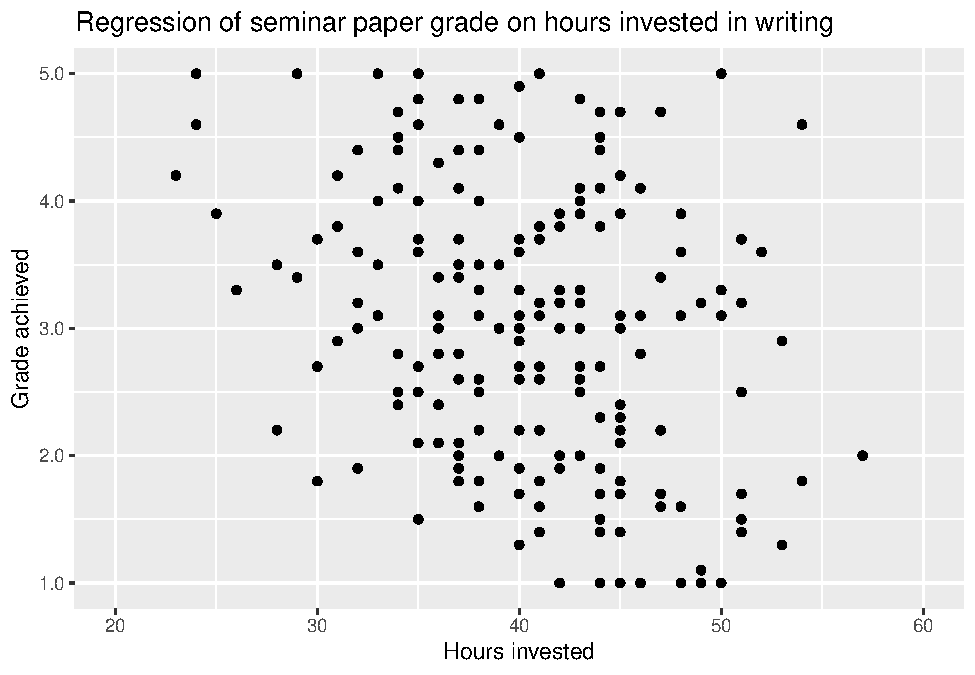
\includegraphics{_main_files/figure-latex/plot_grade_hours-1.pdf}

When we are talking about dependent and independent variables, there is the
convention to plot former on the x-axis and the latter on the y-axis. So the
\emph{y-variable} is to be explained and the \emph{x-variable} is used to explain it.
This convention will also be used in all formulas in this seminar.

Looking at the plot we first see a cloud of dots, representing all combinations
of \texttt{hours} and \texttt{grade} in all our \(200\) observations. It may be hard to pick out
any pattern, but looking closely we can observe that overall the dots seem to
follow a downward slope from the upper left - indicating few hours worked and a
worse grade - towards the lower right - indicating more invested hours and a
better grade. This would be the relationship stated in our hypotheses. The more
hours a student works on a seminar paper the better the final grade will be.

We can try to describe this pattern by adding a line from the upper left to the
lower right.

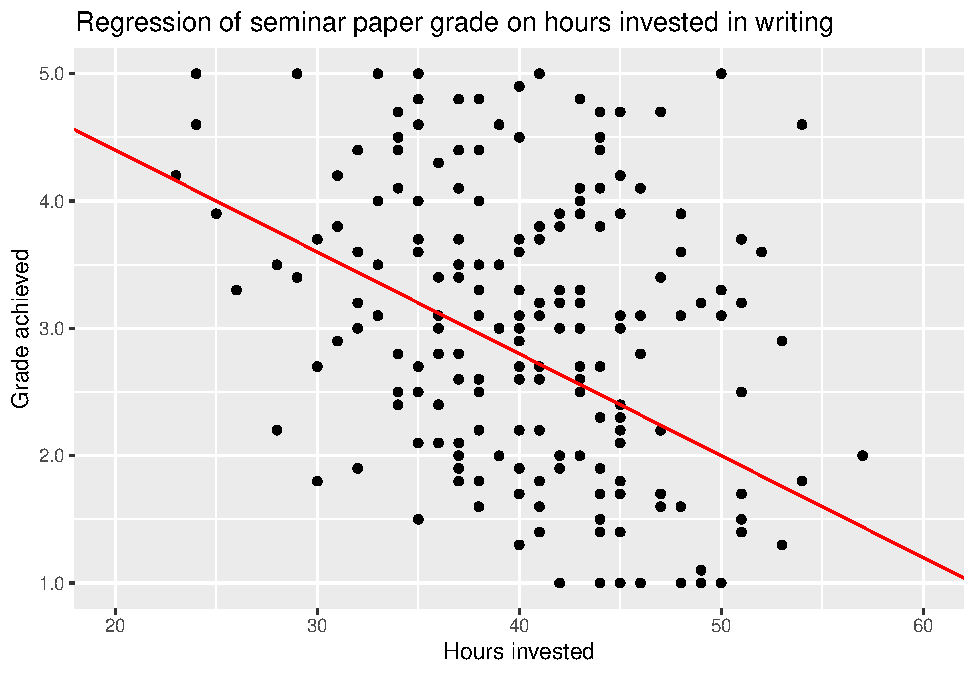
\includegraphics{_main_files/figure-latex/plot_grade_hours_wild_guess-1.pdf}

This describes the realtionship between the two variables as linear. Each hour
invested decreases the grade by a certain amount, for this proposed line by
exactly \(0.08\) points. Remember that decreasing the value of the grade actually
means getting a better grade.

But is this the only possible line or even the \emph{correct} one? Most certainly not
as the values used to draw the line were only a wild guess by the authors. We
could imagine several other lines that also look more or less reasonable - as
well as some that look unreasonable - and add them to the plot.

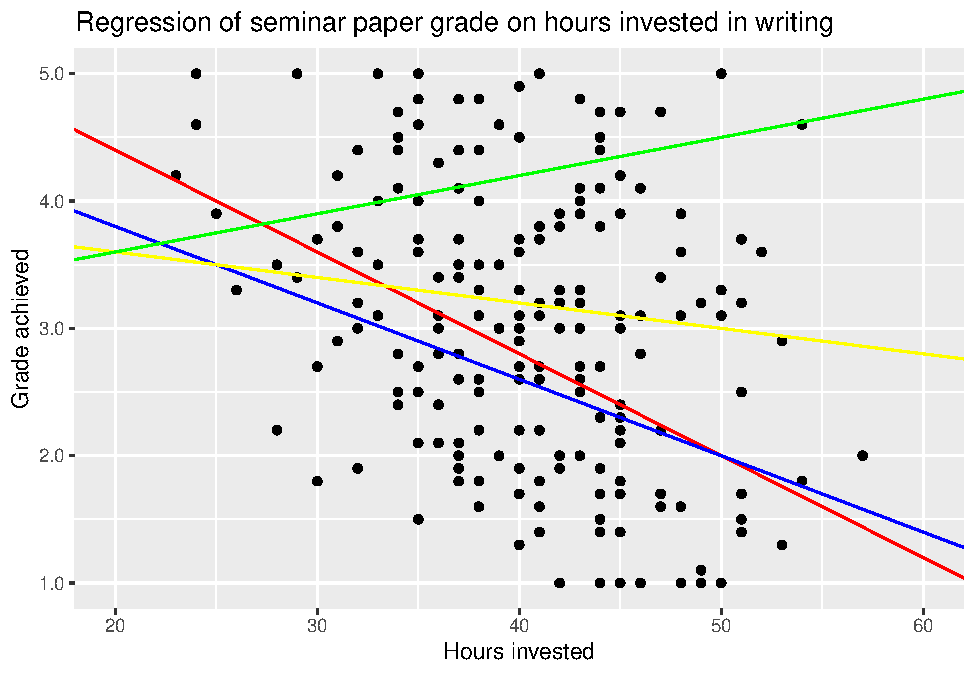
\includegraphics{_main_files/figure-latex/plot_grade_hours_wild_guesses-1.pdf}

While we have some intution, that especially the green line misses the mark by a
lot, we can't really decide between the others just by looking at the plot. The
data points are way to dispersed to see the relationship clearly.

The goal of using a simple linear regression model is to identify the \emph{one} line
that describes the relationship the best. The \emph{best} meaning, with as little
error as possible.

XXX OVERLAPPING DOTS? XXX

\hypertarget{regression-formula}{%
\subsection{Regression Formula}\label{regression-formula}}

To understand how these lines in the above plot were conceived and how to find
the line with the best \emph{fit}, i.e.~the lowest error, we have to understand the
formular for linear regression. While formulas may always be kind of daunting,
we are in luck as tis particular one is actually quite easy to understand,
especially when paired with a graphical representation.

\[y = \beta_0 + \beta_1*x_1 + \epsilon\]

Let us first look at the parts we already know. \(y\) is the dependent variable,
in our case the grade achieved. So one thing is for sure, the whole right part
of the equation has to be used to calculate the value of \(y\) from the data, i.e.
the dependent variable \(x\). Here we have three terms. Let us skip the first one
for now and focus on the second one \(\beta_1*x_1\).

\(x_1\) is the dependent variable, in our case \texttt{hours}. \(\beta_1\) is the
\emph{redression coefficient} for \(x_1\). This value gives us the \emph{slope} of the
regression line. Based on this, we can start rewriting the general formula and
tailor it to our specific use case.

\[y_{grade} = \beta_0 + \beta_{hours}*x_{hours} + \epsilon\]

Let us return to the first wild guess we made above.

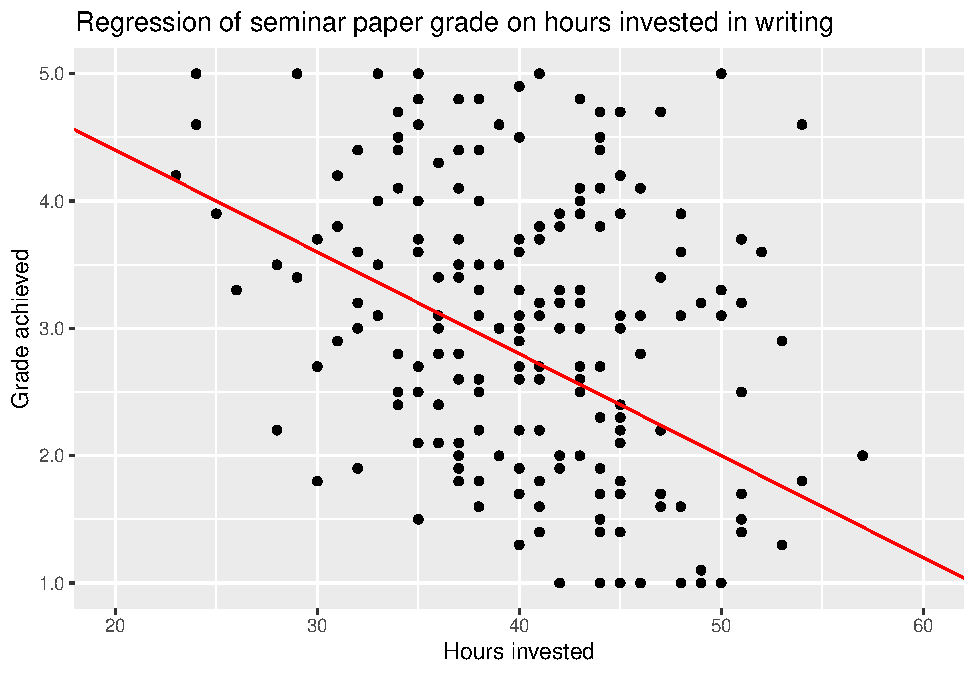
\includegraphics{_main_files/figure-latex/plot_grade_hours_wild_guess_expl_slope-1.pdf}

Here we guessed, that an increase in time invested of one hour decreases the
value of \texttt{grade} by \(0.08\). This is the slope of the red line and thus also the
coefficient in the regression formula that is used in computing said line. So,
\(\beta_{hours} = -0.08\). We can insert this value into our formula.

\[y_{grade} = \beta_0 -0.08*x_{hours} + \epsilon\]

In this way the value of \(x_{hours}\) is multiplied by \(-0.08\). Let us assume a
student worked \(40\) hours on their paper. \(-0.08*40\) being \(-3.2\), we know, that
working 40 hours on a paper \emph{on average} - more on that later - leads to a \(3.2\)
lower grade value and thus a better grade. But \(3.2\) lower than what?

Looking at the formula again, we see that subtract this value from \(\beta_0\).
This is the \emph{intercept}, the value at which the line intersects with the y-axis.
Let us zoom out on our plot, to see what happens.

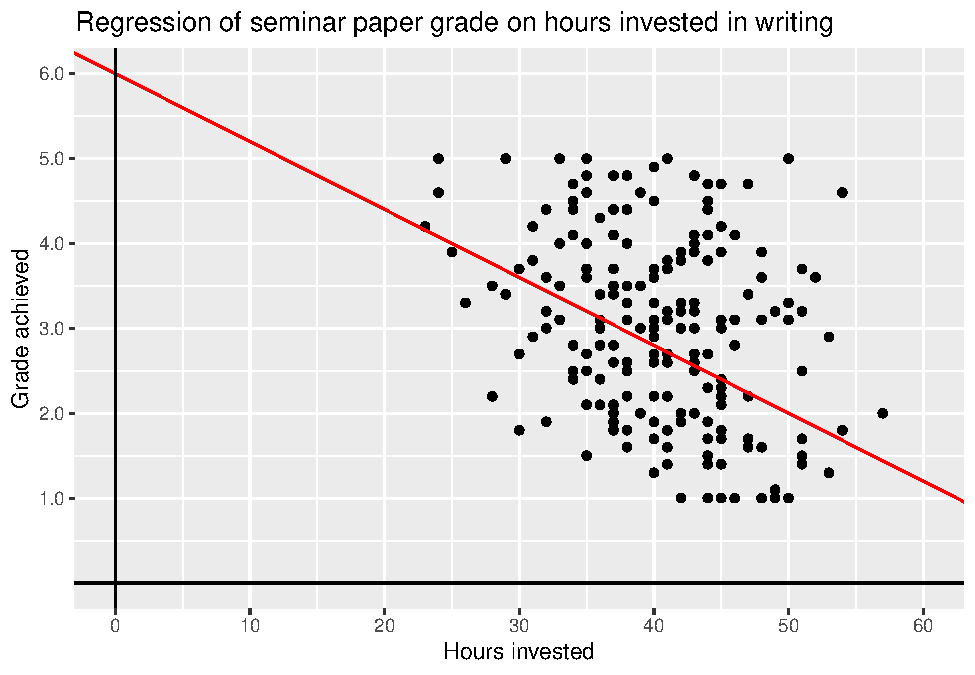
\includegraphics{_main_files/figure-latex/plot_grade_hours_wild_guess_expl_intercept-1.pdf}

We can now see the point where the red line intersects with the y-axis. This is
the intercept of this line, i.e.~\(\beta_0 = 6\).

\[y_{grade} = 6 -0.08*x_{hours} + \epsilon\]

If we now again assume a time investment of \(40\) hours, we can compute
\(6-0.08*40 = 2.8\). So our red regression line - which is still only a wild guess
- assumes, that working 40 hours on a seminar paper will result in a grade of
\(2.8\), on avarage. We can mark these values in our plot

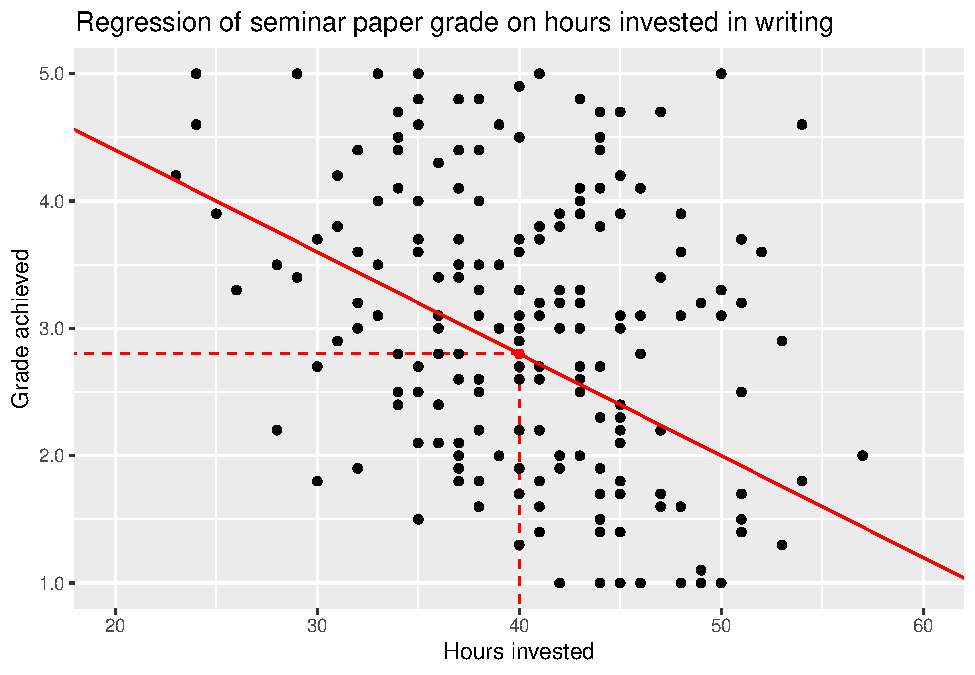
\includegraphics{_main_files/figure-latex/plot_grade_hours_wild_guess_expl_40hours-1.pdf}

The red dot is the intersection of the values \texttt{hours\ =\ 40} and \texttt{grade\ =\ 2.8}.
As this is the value for \(y\) our regression line assumes a student with a time
investment of 40 hours achieves, the red dot also lies exactly on the red line.

But if we look at the plot once again, we can see that most actual observations
for students that invested 40 hours do not actually lie on the regression line
but are scattered above and below the line. So some of these students achieve
much worse or much better grades than \(2.8\) investing the same amount of time in
their work. This leads us to the last part of the formula, \(\epsilon\).

This is the \emph{error term}. Having data that is dispersed like this - and any real
world data will always be - our linear line will never be able to pass exactly
through every data point. Some points may lie exactly on the line, but many or
most will not.

We can visualize this. To keep the plot readable, we only do this for some
random observations but in reality the distance of every data point from the
regression line is taken into account.

\begin{verbatim}
## # A tibble: 5 x 7
##   grade hours previous_grades attendance contact    previous_grades_centered
##   <dbl> <int>           <dbl> <lgl>      <fct>                         <dbl>
## 1   2.3    45             2.6 TRUE       No contact                   -0.335
## 2   1.9    44             2.8 TRUE       In Person                    -0.135
## 3   3.1    38             3.7 TRUE       In Person                     0.765
## 4   3.3    40             3.4 TRUE       E-Mail                        0.465
## 5   4.6    54             4.5 TRUE       No contact                    1.56 
## # i 1 more variable: hours_centered <dbl>
\end{verbatim}

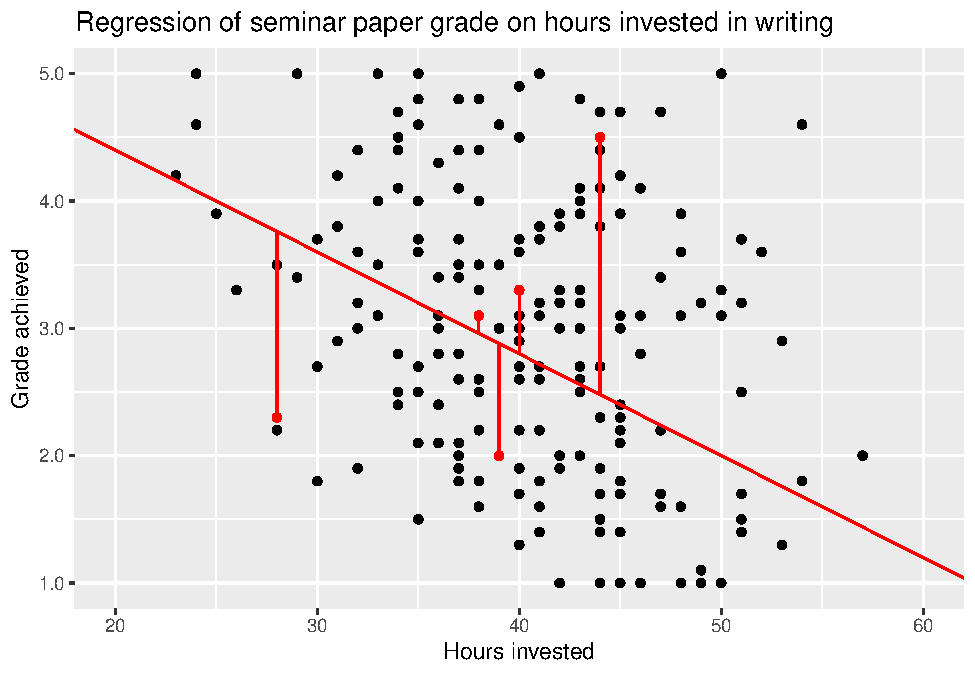
\includegraphics{_main_files/figure-latex/plot_grade_hours_wild_guess_expl_residuals-1.pdf}

The distance of these or rather all points from the line, the \emph{residuals}, are
represented in the error term \(\epsilon\). It is a measure for how wrong our line
is in describing the data in it's entirety. So why is it wrong? We can not say
for sure, but there are two common main reasons.

For one, there may be other variables that also influence the relationship
between invested hours and achieved grade, something that we will return to
later in this session when we expand the idea of linear regression to multiple
independent variables.

But there is also random variation present in every bit of real world data.
While our data is simulated we also added random variation on purpose. Because
this is what real world data is, it's messy and it's noisy.

Not every seminar paper that had the same time investment, e.g.~40 hours, will
have the same quality in results. There may be other influential variables, e.g.
the student's general skill level or if they sought assistance by their lecturer
in preparing the paper, influencing the final grade. But even if the quality of
the paper after working 40 hours would be the same for each student, measurement
error, i.e.~noise, will be introduced because not every lecturer will grade
exactly the same or maybe because papers were submitted at different time
points and grading standards may have changed. If we can not measure these
variables we have to accept these unobservable sources of noise and hope, where
\emph{hope} actually means thorough theoretical and methodical thinking, that we can
still measure our effect of interest. But his also means, that measuring and
modelling \textbf{always} includes uncertainty. We never know for certain if and to
what extent our results are influenced by unobservable variables and random
variation. Still, there are ways to assess this uncertainty, which we will
regularly return to during the course. This should not stop quantitative
social scientists from making strong or even bold arguments based in thorough
theoretical thinking and responsible data analysis, but we always have to
acknowledge the uncertainty included in every step and make it a part of our
interpretations and conclusions.

XXX MAYBE SHORTEN THE SERMON\ldots{} XXX

The error term \(\epsilon\) is the final piece of the puzzle in actually computing
a linear regression model. Without jumping into the mathematics of it all, the
technique that is used to estimate the coefficients \(\beta_0\) and \(\beta_1\) is
called \emph{OLS} - Ordinary Least Squares. What it basically does, is to take the
squares of all residuals, i.e.~the distances of the data points from the
regression line, sum them up and minimise this value. All this substantialy
means is, that OLS searches the regression line with lowest amount of error,
i.e.~the lowest overall distance from the actual data points.

This computation gives us estimates for the regression coefficients in this
formula:

\(\hat{y} = b_0 +b_1*x_1\)

We can see two differences to the formula we started with. First, we write
\(\hat{y}\) - pronounced as ``y hat'' - instead of \(y\). At the same time, we exclude
the error term \(\epsilon\). This means that we are no longer computing the actual
value of \(y\), as in the point on the regression line for a certain value of
\(x_1\) \(+\) the error, but the estimate \(\hat{y}\), as in the point on the
regression line that is predicted for a certain value of \(x_1\). Second, we write
\(b\) instead of \(\beta\). This also alludes to the fact that we are now
computing an estimate for the coefficients based on the data available and not
the real and unknown value of \(\beta\).

XXX MAYBE ALSO SOME CUTTING REQUIRED XXX

XXX include ``on average'' XXX

\hypertarget{regressing-grade-on-hours}{%
\subsection{\texorpdfstring{Regressing \texttt{grade} on \texttt{hours}}{Regressing grade on hours}}\label{regressing-grade-on-hours}}

Now that we have a firmer understanding on what linear regression actually is
and does, we can finally get to the fun part and use the technique for
estimating the effect of \texttt{hours} on \texttt{grade} or in other words, regress
\texttt{grade} on \texttt{hours}.

\begin{verbatim}
## 
## Call:
## lm(formula = grade ~ hours, data = grades)
## 
## Residuals:
##      Min       1Q   Median       3Q      Max 
## -1.88006 -0.83961 -0.08006  0.77006  2.53881 
## 
## Coefficients:
##             Estimate Std. Error t value Pr(>|t|)    
## (Intercept)  5.07912    0.47306  10.737  < 2e-16 ***
## hours       -0.05236    0.01159  -4.517 1.07e-05 ***
## ---
## Signif. codes:  0 '***' 0.001 '**' 0.01 '*' 0.05 '.' 0.1 ' ' 1
## 
## Residual standard error: 1.028 on 198 degrees of freedom
## Multiple R-squared:  0.09344,    Adjusted R-squared:  0.08886 
## F-statistic: 20.41 on 1 and 198 DF,  p-value: 1.075e-05
\end{verbatim}

This is the output from a simple linear regression for \texttt{grade} on \texttt{hours} from
R. How to do this in practice and what the first to lines mean will be the topic
of the next sesion. For now we will focus on the coefficient block and
introduce the additional elements of the output on by one during this session.

The column \texttt{Estimate} gives us the values for \(\beta_0\) and \(\beta_1\) discussed
above. The estimated coefficient for \texttt{hours} tells us that out intuition was
right, the more hours a student invests in writing a paper, the better the grade
will be. In this case every additional hour spent on working will decrease the
value of the grade by \(-0.05236\) points. In keeping with the example of a 40
hour workload this leads to a decrease of \(-0.05236 * 40 = -2.0944\) points.
Adding the intercept from the same column, the estimated grade after working 40
hours is \(5.07912 -0.05236 * 40 = 2.98472\). So on average a student from our
simulated data set will pass after 40 hours of work but will not get a great
grade.
Remember, this is the expected average value. This does not mean that some
students will not get better or worse grades, or even fail to pass, after this
amount of time investment, as we hav seen in the plot.

Now that we know the coefficients for the regression line with the best fit,
i.e.~the lowest error, we can again visualise the result.

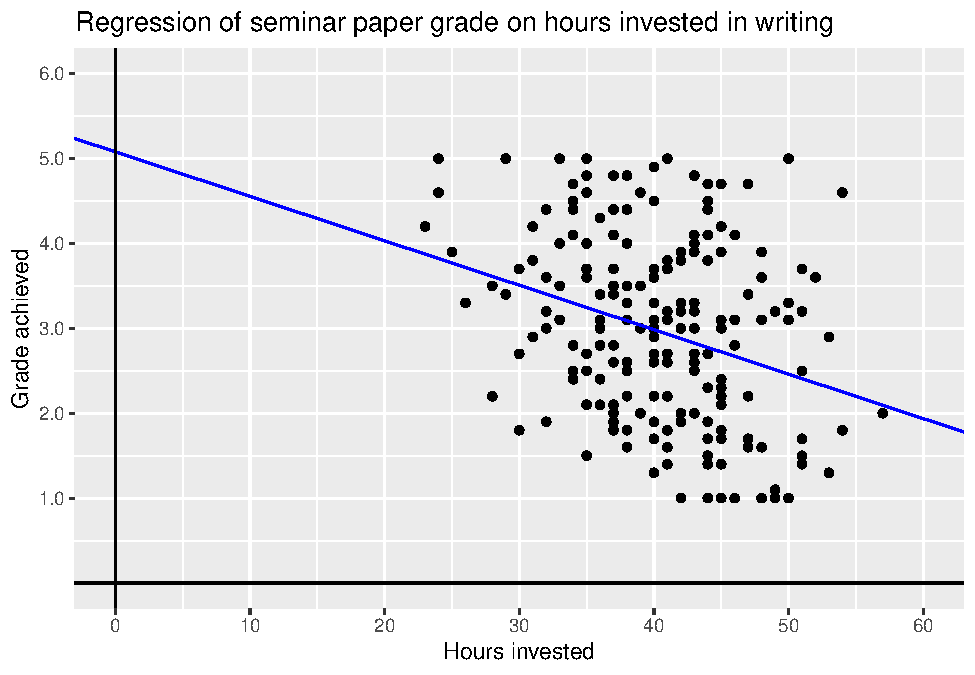
\includegraphics{_main_files/figure-latex/plot_lm_grade_hours-1.pdf}

Now, what grade can a student expect, on average, if they invest exactly 0
hours, i.e.~do nothing and hand in a blank paper. We can look at the graph or to
achieve a more precise result, calculate it.

\[5.07912 -0.05236 * 0 = 5.07912\]

As \(x_{hours} = 0\) for this theoretical example, the estimated value \(\hat{y}\)
or \(y_{grade}\) is the same as the intercept \(\beta_0\). This is what the
intercept represents in general, the estimated value \(\hat{y}\) when the
dependent variable is \(0\).

Now, investing zero hours in a seminar paper is not only not advisable, it is
also not a value we observed in our data. If the data would include observations
with zero hours of time invested, the grade would be a firm \(5.0\) and the same
would be true for low single digits, i.e.~turning in a two-pager as a seminar
paper. The takeaway is, that the model is highly dependent on the data that it
is trained on. If the data would have included such cases we could expect a
higher intercept and a steeper slope, i.e.~stronger negative coefficient.

Luckily all our simulated students have put in at least some hours. But as we do
not have data for zero to \(22\) hours, we can not really make reliable estimates
in this range. Because of this, it does not really make sense to enter \texttt{hours}
into the regression model as ranging from \(0\) to \(57\). One solution that is
often used for metric variables is to center them on their mean. This can be
achieved by simply subtracting the mean of \(x\) from each individual value:
\(x_i - \bar{x}\).

We can now rerun the regression.

\begin{verbatim}
## 
## Call:
## lm(formula = grade ~ hours_centered, data = grades)
## 
## Residuals:
##      Min       1Q   Median       3Q      Max 
## -1.88006 -0.83961 -0.08006  0.77006  2.53881 
## 
## Coefficients:
##                Estimate Std. Error t value Pr(>|t|)    
## (Intercept)     2.96750    0.07267  40.835  < 2e-16 ***
## hours_centered -0.05236    0.01159  -4.517 1.07e-05 ***
## ---
## Signif. codes:  0 '***' 0.001 '**' 0.01 '*' 0.05 '.' 0.1 ' ' 1
## 
## Residual standard error: 1.028 on 198 degrees of freedom
## Multiple R-squared:  0.09344,    Adjusted R-squared:  0.08886 
## F-statistic: 20.41 on 1 and 198 DF,  p-value: 1.075e-05
\end{verbatim}

Comparing the results to the first model shows us, that the coefficient for
\(b_{hours\_centered}\) is exactly the same as for \(b_{hours}\). So the effect
of working more hours has not changed. What has changed is the value of the
intercept. This will make more sense if we again plot the regression line.

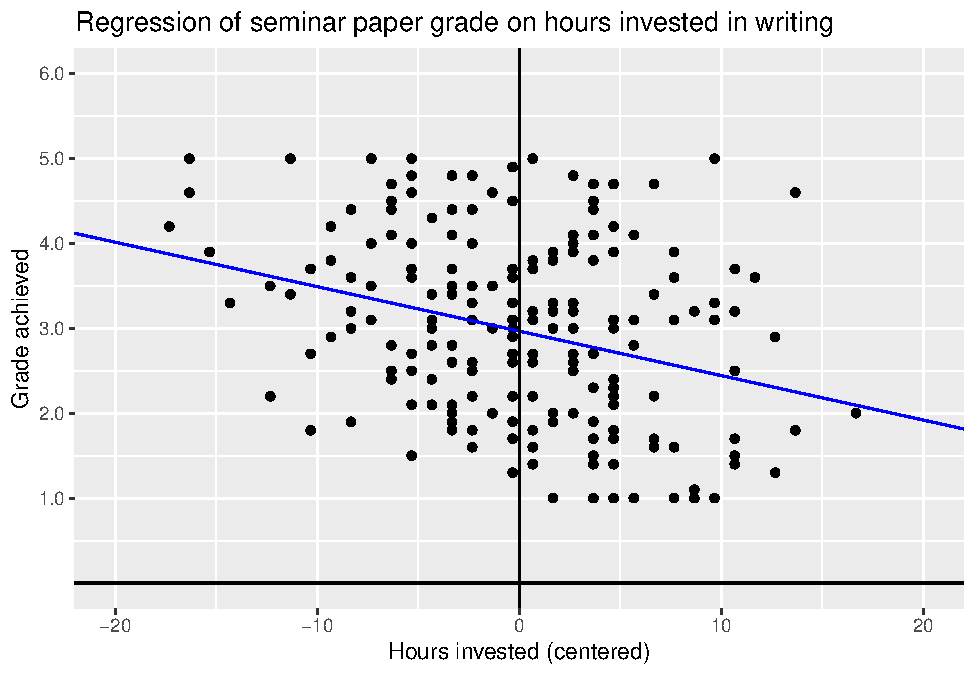
\includegraphics{_main_files/figure-latex/plot_lm_grade_hours_centered-1.pdf}

By centering the x-Variable on its mean we have changed its interpretation.
A value of \texttt{hours\ =\ 0} now stands for investing as much time as is the mean
of \texttt{hours} in the whole data set, which in this case is \(40.33\) hours. Positive
values indicate that a student worked \(x\) hours more, negatives indicate \(-x\)
hours less compared to the mean. In this way, we also moved the y-axis and thus
changed the interpretation of the intercept. Its new value of \(2.9675\) now
indicates the estimate for a student who invests the mean value of \texttt{hours} in
their work, i.e.~\(40.33\). We will use this version of the variable for the rest
of the session.

\hypertarget{multiple-linear-regression}{%
\section{Multiple Linear Regression}\label{multiple-linear-regression}}

Maybe explaining the grade a student receives solely based on the hours of
invested time, does not paint the whole picture. As we have alluded to, there
may be other variables that could also have an effect of the final grade.

A \emph{simple linear regression} only allows for one independent variable. This is
why we need \emph{multiple linear regression} if we want to start introducing
additional variables into the model. Luckily this is easy to understand as we
already know the formula for a simple linear regression.

\[y = \beta_0 + \beta_1*x_1 + \epsilon\]

To change a simple into a multiple linear regression, we just start adding the
additional variables and their coefficients additively to the formula.

\[y = \beta_0 + \beta_1*x_1 + \beta_2*x_2 + ... + \beta_k*x_k + \epsilon\]

So to add a second variable and its coeffcient we add the term \(+ \beta_2*x_2\)
and so on until we added all independent varibles of interest \(k\) to the model.
Everything else works exactly as described above for the simple model.

\hypertarget{adding-additional-variables}{%
\subsection{Adding additional variables}\label{adding-additional-variables}}

We already expected that the mean of the previous grades could be a strong
predictor for future grades. We could understand these as a \emph{proxy} variable for
the general skill level of a student. The higher the skill level, the higher
previous grades will have been.

How we can add additional variables in R code will again be a topic for the next
session, but let us look at the results of a regression of \texttt{grade} on
\texttt{hours\_centered} and \texttt{previous\_grades\_centered}, the latter being centered on the
mean previous grade of \(2.935\).

\begin{verbatim}
## 
## Call:
## lm(formula = grade ~ hours_centered + previous_grades_centered, 
##     data = grades)
## 
## Residuals:
##      Min       1Q   Median       3Q      Max 
## -1.44462 -0.30556  0.00622  0.32878  1.31002 
## 
## Coefficients:
##                           Estimate Std. Error t value Pr(>|t|)    
## (Intercept)               2.967500   0.038316  77.449   <2e-16 ***
## hours_centered           -0.056543   0.006114  -9.248   <2e-16 ***
## previous_grades_centered  0.904079   0.039830  22.699   <2e-16 ***
## ---
## Signif. codes:  0 '***' 0.001 '**' 0.01 '*' 0.05 '.' 0.1 ' ' 1
## 
## Residual standard error: 0.5419 on 197 degrees of freedom
## Multiple R-squared:  0.7492, Adjusted R-squared:  0.7467 
## F-statistic: 294.3 on 2 and 197 DF,  p-value: < 2.2e-16
\end{verbatim}

As we added a new variable, we now see three coefficients.
The intercept has not changed. It now indicates the estimated grade for a
student who invests the mean amount of hours, \(40.33\), and whose previous grades
are exactly \(2.935\).

The coefficient for \texttt{hours\_centered} got mildly more negative, still telling us
that the value of \texttt{grade} gets lower, the more hours are invested in writing the
paper. This coefficient now gives us the effect while \emph{controlling} for the
effect of \texttt{previous\_grades\_centered}. This is what multiple linear regression
does, giving us the coefficients for our variables of interest while keeping all
other independent variables at specific values. As we have centered the variable
for previous grades, the coefficient for \texttt{hours\ centered} gives us the effect
when the previous grades were exactly at the mean of \(2,935\).

In the same way, the coefficient for \texttt{previous\_grades\_centered} gives us the
effect of previous grades when the invested hours are controlled for, in this
case when the invested hours were exactly \(40.33\). The coefficient is rather
high and positive. This indicates that a student with a previous grade value
that is \(1\) above the mean, is estimated to receive a new grade that is \(0.9\)
points above the intercept. This means, that the previous grade is a very strong
predictor for the new grade.

While plotting in more than two dimensions gets really hard, we can still
calculate \(\hat{y}\) for certain values of both independent variables.
We already know the predicted grade for a student with mean values on both
independent variables, as this is the intercept. To make sure that we correct,
we can calculate it again.

\[b_0 + b_{hours\_centered}*0 + b_{previous\_grades\_centered}*0 = 2.9675\]

For this case we can see, that the previous grade actually is a strong
predictor, as the previous and new grades are substantially the same.

What if a student whose previous grades were \(1\) above the mean, so just below
\(4.0\) but who decides to invest \(10\) hours more than the mean for the new paper?

\[2.9675 - 0.056543 * 10 + 0.904079 * 1 = 3.306149\]

So the good message is, while previous grades are a strong predictor, putting in
more hours still leads to better grades.

What if a really good student decides to rely on their skill and to work less
this time?

\[2.9675 - 0.056543 * -10 + 0.904079 * -2 = 1.724772\]

While \(1.7\) is still a very good grade, working 10 less hours than the mean of
students leads to a substantially worse estimate compared to the about \(1.0\)
received in previous grades.

\hypertarget{adding-dummy-variables}{%
\subsection{Adding dummy variables}\label{adding-dummy-variables}}

Another variable that could be of interest in explaining the received grade,
is if a student attended most of the seminar sessions.
\texttt{attendance} holds this information in the form of a dummy variable. Dummies can
only have two states. ``Yes'' or ``No'', ``1'' or ``0'' or in this case ``\texttt{TRUE}'' or
``\texttt{FALSE}''.

Let us add the variable to our model.

\begin{verbatim}
## 
## Call:
## lm(formula = grade ~ hours_centered + previous_grades_centered + 
##     attendance, data = grades)
## 
## Residuals:
##      Min       1Q   Median       3Q      Max 
## -1.41059 -0.30910  0.01667  0.35607  1.29849 
## 
## Coefficients:
##                           Estimate Std. Error t value Pr(>|t|)    
## (Intercept)               3.157411   0.078658  40.141  < 2e-16 ***
## hours_centered           -0.053942   0.006088  -8.860 4.85e-16 ***
## previous_grades_centered  0.911802   0.039282  23.212  < 2e-16 ***
## attendanceTRUE           -0.248250   0.090246  -2.751   0.0065 ** 
## ---
## Signif. codes:  0 '***' 0.001 '**' 0.01 '*' 0.05 '.' 0.1 ' ' 1
## 
## Residual standard error: 0.5331 on 196 degrees of freedom
## Multiple R-squared:  0.7586, Adjusted R-squared:  0.7549 
## F-statistic: 205.3 on 3 and 196 DF,  p-value: < 2.2e-16
\end{verbatim}

This gives us a new line in the R Output holding an estimate for
\texttt{attendanceTRUE}. What is meant by this? In contrast to the metric variables we
have uses in our model up to this point, a dummy variable - or binary variable -
can only have two states. As we are using a logical variable here, it can only
have the value \texttt{TRUE} - here indicating regular attendance - or \texttt{FALSE}. So what
the output shows us, is the effect of attendance being \texttt{TRUE} compared to being
\texttt{FALSE}. If a student did regularly attend the seminar, the estimated grade is
\(-0.248250\) lower compared to when they did not.

We can observe what happens in the formula:

\[\hat{y} = b_0 + b_{hours\_centered}*x_{hours\_centered} + b_{previous\_grades\_centeterd}*x_{previous\_grades\_centeterd} + b_{attendance} * x_{attendance}\]

If you calculate with \texttt{TRUE} and \texttt{FALSE} in R, the values \(1\) and \(0\) are used
respectively. So \(x_{attendance}\) can either have the value \(1\) for regular
attendance or \(0\) for not so regular attendance.

If a student did regularly attend, the coefficient \$b\_\{attendance\} becomes a
part of the estimate \(\hat{y}\):

\[\hat{y} = b_0 + b_{hours\_centered}*x_{hours\_centered} + b_{previous\_grades\_centeterd}*x_{previous\_grades\_centeterd} + b_{attendance} * 1\]

If stduent did not regularly attended, this happens:

\[\hat{y} = b_0 + b_{hours\_centered}*x_{hours\_centered} + b_{previous\_grades\_centeterd}*x_{previous\_grades\_centeterd} + b_{attendance} * 0\]
\[\hat{y} = b_0 + b_{hours\_centered}*x_{hours\_centered} + b_{previous\_grades\_centeterd}*x_{previous\_grades\_centeterd}\]

The coeeffcient is no longer a part of the estimate. One can basically say, the
coefficient gets switched on or off by the value of the dummy variable.

So while the estimate for a student with mean values for invested hours and
previous grades who did not attend is the intercept of \(3.157411\) for the same
student with attendance we can calculate the estimate as:

\[3.157411 - 0.053942*0 + 0.911802*0 - 0.248250 * 1 = 3.157411 - 0.248250 = 2.909161\]

It seems attending class is an easy way to raise one's grades.

\hypertarget{adding-categorical-variables}{%
\subsection{Adding categorical variables}\label{adding-categorical-variables}}

We have one further variable in our simulated data set that could be of interest
in explaining, what makes a good grade in a seminar paper.\texttt{contact} is a factor
variable. It can take three different categories. \texttt{No\ contact} indicates that
the student did not contact the lecturer to discuss a research question or the
laid out plan for the paper. \texttt{E-Mail} means that there was some written contact
and at least the basics for the paper were discussed before writing. Lastly,
\texttt{In\ Person} stands for an in depth discussion with the lecturer, clearing up
problems beforehand and having a more stringent vision for the paper before
writing the first word.

Let us add the variable to our model.

\begin{verbatim}
## 
## Call:
## lm(formula = grade ~ hours_centered + previous_grades_centered + 
##     attendance + contact, data = grades)
## 
## Residuals:
##     Min      1Q  Median      3Q     Max 
## -1.3835 -0.2525  0.0167  0.2678  0.9347 
## 
## Coefficients:
##                           Estimate Std. Error t value Pr(>|t|)    
## (Intercept)               3.617949   0.068077  53.145  < 2e-16 ***
## hours_centered           -0.050830   0.004433 -11.466  < 2e-16 ***
## previous_grades_centered  0.874123   0.028657  30.503  < 2e-16 ***
## attendanceTRUE           -0.324653   0.065781  -4.935 1.72e-06 ***
## contactE-Mail            -0.413808   0.069817  -5.927 1.39e-08 ***
## contactIn Person         -0.853252   0.063964 -13.340  < 2e-16 ***
## ---
## Signif. codes:  0 '***' 0.001 '**' 0.01 '*' 0.05 '.' 0.1 ' ' 1
## 
## Residual standard error: 0.3869 on 194 degrees of freedom
## Multiple R-squared:  0.8741, Adjusted R-squared:  0.8709 
## F-statistic: 269.4 on 5 and 194 DF,  p-value: < 2.2e-16
\end{verbatim}

Wait, we entered three categories into the model and got estimates for two of
them. What happened? What R does is to create two dummy variables on the fly.
The first discerns between having E-Mail contact or no contact at all. The
second one between having contact in person to no contact at all. So for
categorical variables in regression models we always compare being in one
category to being in the \emph{base category}. In this case the base category is
\texttt{No\ contact} but we could also change the base category. It depends on what we
are interested in comparing to. For our example comparing the effects of having
more in depth contact to having none makes sense.

Let us look at our formula again:

\[\hat{y} = b_0 + b_{hours\_centered}*x_{hours\_centered} + b_{previous\_grades\_centeterd}*x_{previous\_grades\_centeterd} + b_{attendance} * x_{attendance} + b_{E-Mail} * x_{E-Mail} + b_{In Person} * x_{In Person}\]

Now there are three possibilities. A student can have no contact at all. In this
case both dummy variables equal \(0\). To make our formula easier to read, we have
abbreviated the middle part for now:

\[\hat{y} = b_0 + ... + b_{E-Mail} * 0 + b_{In Person} * 0\]
So in this case, controlling all other independent variables at their default
values, the mean for the metric variables, \texttt{FALSE} for \texttt{attendance}, the
intercept gives us the estimate for the grade as both dummy variables that
were created for \texttt{contact}are ``switched off''.

THe two other possibilities are that a student either had E-Mail contact or an
in person discussion:

\[\hat{y} = b_0 + ... + b_{E-Mail} * 1 + b_{In Person} * 0\]

\[\hat{y} = b_0 + ... + b_{E-Mail} * 0 + b_{In Person} * 1\]

In both cases the relevant dummy variable is ``switched on'' while the other does
not factor into the equation.

Looking at the estimates, we can see that having contact to the lecturer before
writing has strong negative effects, resulting in better grades. Having E-Mail
contact reduces the value of \texttt{grade} by \(-0.413808\) points, having an in person
discussion by \(-0.853252\).

So what grade can a student whose previous grades were at the mean of \(2.935\),
but who decided to put in 20 hours more compared to their peers, regularly
attend the seminar and have an in-depth personal discussion before writing their
paper expect on average as their new grade?

\[3.617949 - 0.050830 * 20 + 0.874123 * 0 - 0.324653 * 1 - 0.413808 * 0 - 0.853252 * 1 = 1.423444\]

Putting in the hours, attending and working with your lecturer seems to pay off,
at least in our simulated data set.

\hypertarget{returning-to-our-research-question}{%
\section{Returning to our research question}\label{returning-to-our-research-question}}

Our examplary research question concerned itself with what makes a good grade in
a seminar paper. In particular we were interested in the effect of the invested
hours, as our main hypothesis was that more hours lead to better grades. What do
we know now?

All analysis point towards a clear effect from \texttt{hours} on \texttt{grade}. This effect
was consistently visible in all of our models. But did we correctly identify
and estimate the effect of interest? Maybe. The problem is, we actually did not
approach the analysis correctly. In a real analysis we should \textbf{absolutely}
refrain from adding variables to our model that \emph{could be} relevant until we are
satisfied or all available variables are bunched into one huge model. It was
fine to do this in this introduction to linear regression and for learning how
different types of variables can be used in a regression model. But in a real
project, we have to invest time to think about which variables to add because we
assume that they have a relevant effect based on theoretical assumptions about
the processes we are interested in.

So let us do this now and vow do make this our first step in all future
endeavors. While we do not have a clear theoretical basis, we can make clear
assumptions on the data generating process and draw these in a DAG.

\begin{verbatim}
## Warning: package 'dagitty' was built under R version 4.2.3
\end{verbatim}

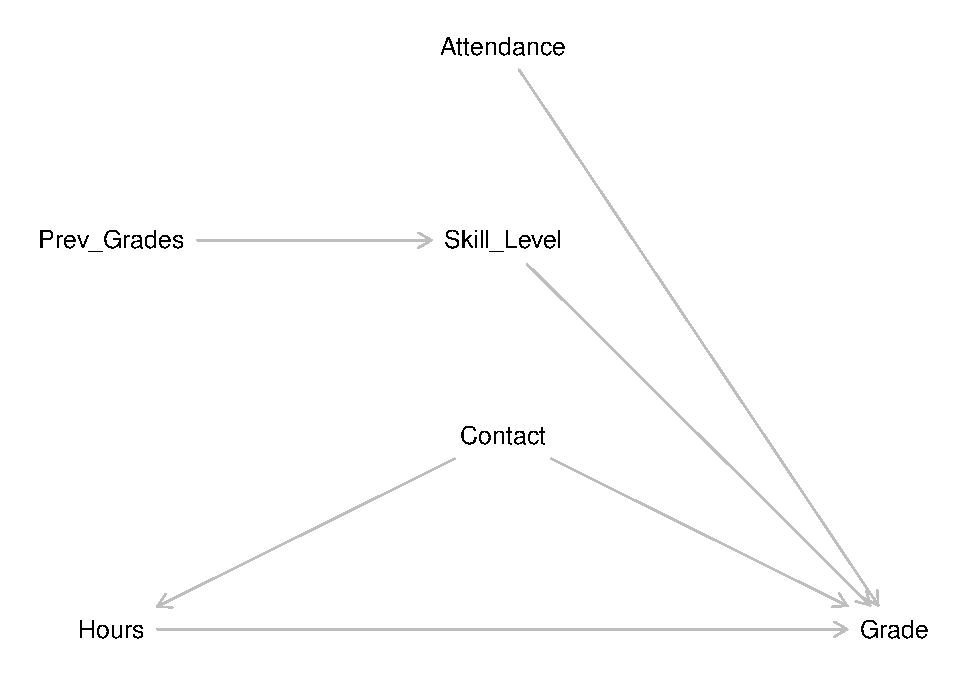
\includegraphics{_main_files/figure-latex/dag-1.pdf}

XXX MAYBE NICEN IT UP XXX

Our central assumption, and the effect we want to identify and estimate, is the
direct effect from \texttt{hours} on \texttt{grade} in the bottom line. The more hours a
student invests, the better the grade should be. This is our variable of
interest and it has to be included in the model.

The assumed effect of \texttt{contact} is more complex. For one we assume that a more
in-depth contact with the lecturer will increase the grade directly. The
research question will be more focused, the student will know what is important
to a certain lecturer, common mistakes can be avoided if they are cleared up
beforehand and so on. But we will also assume that \texttt{contact} will have an effect
on \texttt{hours} in the sense that the hours invested can be used more efficiently if
an in-depth discussion has taken place. Instead of wasting time running into
problems that could have been avoided most of the invested time can actually go
into constructive work. This makes \texttt{contact} a confounder for \texttt{grade} and
\texttt{hours}. Tapping into the knowledge from the last session, now we know that we
also have to control for \texttt{contact} to measure the effect of \texttt{hours} correctly.

A student's skill level will also have a direct effect on \texttt{grade}. As we do not
have a direct measure of skill in our data, we use \texttt{previous\_grades} as a proxy
for skill level. \texttt{attendance} also has a direct effect on \texttt{grade} as students
who were present in the seminar will not only have learned the seminar's
contents, but will also have a better understanding of what is expected in their
seminar papers. As neither skill level - or \texttt{previous\_grades} - nor \texttt{attendance}
has any connection to \texttt{hours} we also should not control for them in our model.

That leaves us with \texttt{hours} and \texttt{contact} to be included in our linear
regression, if our goal is to accuarately identify and estimate the effect of
invested time on the final grade. So let us do this:

\begin{verbatim}
## 
## Call:
## lm(formula = grade ~ hours_centered + contact, data = grades)
## 
## Residuals:
##      Min       1Q   Median       3Q      Max 
## -1.85595 -0.74624 -0.02106  0.66648  2.50161 
## 
## Coefficients:
##                  Estimate Std. Error t value Pr(>|t|)    
## (Intercept)       3.44352    0.10404  33.098  < 2e-16 ***
## hours_centered   -0.04967    0.01052  -4.723 4.43e-06 ***
## contactE-Mail    -0.46482    0.16785  -2.769  0.00616 ** 
## contactIn Person -1.02804    0.15240  -6.746 1.67e-10 ***
## ---
## Signif. codes:  0 '***' 0.001 '**' 0.01 '*' 0.05 '.' 0.1 ' ' 1
## 
## Residual standard error: 0.9305 on 196 degrees of freedom
## Multiple R-squared:  0.2643, Adjusted R-squared:  0.253 
## F-statistic: 23.47 on 3 and 196 DF,  p-value: 5.072e-13
\end{verbatim}

This is our estimate. Each hour invested beyond the mean of \(40.33\) hours
changes the grade by about \(-0.05\) points. This supports our hypotheses and we
can conclude, that investing more hours into writing a seminar paper actually
is a worthwhile investment.

But remember: This is correct as long as our DAG is drawn correctly. This is
always debatable. Maybe we should assume an effect from skill level on \texttt{hours}.
The higher the skill level the more efficiently the available time can be used.
For this example we know the DAG is correct, because we have simulated the data
exactly in this way. For real world applications we never know if our DAG is
correct. All we can - and have to - do is base it on thorough thought,
theoretical work and sound arguments.

This all is true \emph{if} our goal is to estimate an effect of interest as precisely
as possible. But as we have alluded to in the introduction to this session we
could also use modelling with a different goal, i.e.~predicting a grade as
accurately as possible. For this task, the model which only includes \texttt{hours} and
\texttt{contact} will not do the best job. From our DAG we know that \texttt{attendance} and
\texttt{previous\_grade} should have an effect on \texttt{grade}, as we have also seen in our
models. For this task the full model including all these variables will produce
better estimates. We will return to this in a later session, but for now we
should remember that we have to know our task because the task dictates which is
the best model to use.

\hypertarget{maybes}{%
\section{Maybes}\label{maybes}}

\begin{itemize}
\item
  maybe talk about std. errors + p-values -\textgreater{} or next week
\item
  Introduce R\^{}2 and adj here
\item
  Mediation
\item
  maybe theory into DAG session and example into application
\item
  Interactions

  \begin{itemize}
  \tightlist
  \item
    maybe introduce here and apply next session
  \item
    maybe push it all into next session
  \item
    or leave out completely
  \end{itemize}
\item
  Multiple outcomes
\item
  maybe leave out
\end{itemize}

\hypertarget{lin-t-2}{%
\chapter{Linear Regression Theory II: Multiple Linear Regression}\label{lin-t-2}}

Here goes some texts.

\hypertarget{application-of-linear-regression}{%
\section{Application of Linear Regression}\label{application-of-linear-regression}}

\hypertarget{log-t-3}{%
\chapter{Linear Regression Theory III: Diagnostics}\label{log-t-3}}

\hypertarget{introduction-1}{%
\section{Introduction}\label{introduction-1}}

\hypertarget{what-is-linear-regression-1}{%
\section{What is Linear Regression}\label{what-is-linear-regression-1}}

\begin{itemize}
\tightlist
\item
  Part of Generalized Linear Models
\end{itemize}

\hypertarget{when-and-for-what-can-it-be-used}{%
\section{When and for what can it be used?}\label{when-and-for-what-can-it-be-used}}

\begin{itemize}
\item
  Categorical outcome variables
\item
  Predictors can be metric or categorical
\item
  Assumptions
\end{itemize}

\hypertarget{formal}{%
\section{Formal}\label{formal}}

\hypertarget{regression-formula-1}{%
\section{Regression Formula}\label{regression-formula-1}}

\begin{itemize}
\tightlist
\item
  Logistic Regression

  \begin{itemize}
  \tightlist
  \item
    show logistic function (shape)
  \item
    Link function
  \item
    show intercept + beta graphically
  \item
    How to get the coefficients

    \begin{itemize}
    \tightlist
    \item
      super short: ML (graphically not how to solve); maybe leave out
    \end{itemize}
  \end{itemize}
\end{itemize}

\hypertarget{interpretation-of-results}{%
\section{Interpretation of results}\label{interpretation-of-results}}

\begin{itemize}
\tightlist
\item
  Show example from WVS data (without the R code)
\end{itemize}

\hypertarget{maybes-1}{%
\section{Maybes}\label{maybes-1}}

\begin{itemize}
\item
  Mediation
\item
  maybe to hard to do correctly
\item
  khb package available?
\item
  Interactions

  \begin{itemize}
  \tightlist
  \item
    similar problem to above
  \end{itemize}
\item
  Multiple outcomes
\item
  maybe leave out
  \textless\textless\textless\textless\textless\textless\textless{} Updated upstream
\item ~
  \hypertarget{multinomial-logistic-regression}{%
  \chapter{Multinomial logistic regression}\label{multinomial-logistic-regression}}
\item
  Multinomial logistic regression
  \textgreater\textgreater\textgreater\textgreater\textgreater\textgreater\textgreater{} Stashed changes
\end{itemize}

\hypertarget{lin-a}{%
\chapter{Linear Regression - Application}\label{lin-a}}

\hypertarget{example-research-question}{%
\section{Example research question}\label{example-research-question}}

\begin{itemize}
\tightlist
\item
  Short theory

  \begin{itemize}
  \tightlist
  \item
    DAG from this

    \begin{itemize}
    \tightlist
    \item
      What do we have to control for to identify effect of interest?
    \end{itemize}
  \end{itemize}
\end{itemize}

\hypertarget{application-with-wvs-data}{%
\section{Application with WVS data}\label{application-with-wvs-data}}

XXX USING FAKE DATE FOR NOW XXX

\begin{Shaded}
\begin{Highlighting}[]
\FunctionTok{library}\NormalTok{(tidyverse)}
\FunctionTok{load}\NormalTok{(}\StringTok{"grades.RData"}\NormalTok{)}
\end{Highlighting}
\end{Shaded}

\hypertarget{r-code}{%
\subsection{R Code}\label{r-code}}

To conduct a multiple linear regression in R, we can use the built-in \emph{base R}
function \texttt{lm()}. The function is straightforward to use. As the first argument
we write the regression formula in R's \emph{formula syntax}.

In the formula syntac we start by writing the name of our \texttt{dependent\_variable}
followed by a \emph{tilde} \texttt{\textasciitilde{}}. You can read this as an \(=\) or as ``regress the
dependent variable on''. After the tilde we add our first \texttt{indepedent\ variable}
by again writing out its name. If we have multiple independent variables in our
model - so we are runnign a \emph{multiple linear regression} - we can add those by
writing a \texttt{+} followed by the name of the variable to be added.

As a second argument, the function needs the name of the object that holds our
data.

So if we want to regress XXX on XXX, we just write:

\begin{Shaded}
\begin{Highlighting}[]
\FunctionTok{lm}\NormalTok{(grade }\SpecialCharTok{\textasciitilde{}}\NormalTok{ hours\_centered, }\AttributeTok{data =}\NormalTok{ grades)}
\end{Highlighting}
\end{Shaded}

\begin{verbatim}
## 
## Call:
## lm(formula = grade ~ hours_centered, data = grades)
## 
## Coefficients:
##    (Intercept)  hours_centered  
##        2.96750        -0.05236
\end{verbatim}

This gives us a short output. The first line just echoes our code used to run
the regression. We have seen this in the last session already, but now we know
what the meaning was. After this we have a short block with the estimated
coefficients. As we have run a simple linear regression, we only get the
intercept and the coefficient for the sole independent variable used in the
model. If we would have run a multiple linear regression, the result would
basically look the same, only with more coefficients to display.

Before we dive into the results, we should talk about how to receive a more
verbose output that does not hide all the other vital information that is
associated with the model.

The easiest way is to use the base R function \texttt{summary()}. This is a generic R
function that returns different summaries, depending on the object it is used
on. We can for example use it on a data frame or tibble to get some descriptive
statistics for the included variables.

\begin{Shaded}
\begin{Highlighting}[]
\FunctionTok{summary}\NormalTok{(grades)}
\end{Highlighting}
\end{Shaded}

\begin{verbatim}
##      grade           hours       previous_grades attendance     
##  Min.   :1.000   Min.   :23.00   Min.   :1.000   Mode :logical  
##  1st Qu.:2.100   1st Qu.:36.00   1st Qu.:2.300   FALSE:47       
##  Median :3.000   Median :41.00   Median :2.950   TRUE :153      
##  Mean   :2.967   Mean   :40.33   Mean   :2.935                  
##  3rd Qu.:3.725   3rd Qu.:45.00   3rd Qu.:3.625                  
##  Max.   :5.000   Max.   :57.00   Max.   :5.000                  
##        contact   previous_grades_centered hours_centered  
##  No contact:80   Min.   :-1.935           Min.   :-17.33  
##  E-Mail    :50   1st Qu.:-0.635           1st Qu.: -4.33  
##  In Person :70   Median : 0.015           Median :  0.67  
##                  Mean   : 0.000           Mean   :  0.00  
##                  3rd Qu.: 0.690           3rd Qu.:  4.67  
##                  Max.   : 2.065           Max.   : 16.67
\end{verbatim}

When we use \texttt{summary()} on a model object, like the one created by \texttt{lm()}, we
get a different output. Before we apply this we should save our model in an
object. This is good practice in most cases as we can now apply all additional
analysis of the model on ths object and we do not have to rerun the model
every time.

\begin{Shaded}
\begin{Highlighting}[]
\NormalTok{m1 }\OtherTok{\textless{}{-}} \FunctionTok{lm}\NormalTok{(grade }\SpecialCharTok{\textasciitilde{}}\NormalTok{ hours\_centered, }\AttributeTok{data =}\NormalTok{ grades)}
\end{Highlighting}
\end{Shaded}

We can now apply \texttt{summary()} on the object \texttt{m1}, short for ``model 1'':

\begin{Shaded}
\begin{Highlighting}[]
\FunctionTok{summary}\NormalTok{(m1)}
\end{Highlighting}
\end{Shaded}

\begin{verbatim}
## 
## Call:
## lm(formula = grade ~ hours_centered, data = grades)
## 
## Residuals:
##      Min       1Q   Median       3Q      Max 
## -1.88006 -0.83961 -0.08006  0.77006  2.53881 
## 
## Coefficients:
##                Estimate Std. Error t value Pr(>|t|)    
## (Intercept)     2.96750    0.07267  40.835  < 2e-16 ***
## hours_centered -0.05236    0.01159  -4.517 1.07e-05 ***
## ---
## Signif. codes:  0 '***' 0.001 '**' 0.01 '*' 0.05 '.' 0.1 ' ' 1
## 
## Residual standard error: 1.028 on 198 degrees of freedom
## Multiple R-squared:  0.09344,    Adjusted R-squared:  0.08886 
## F-statistic: 20.41 on 1 and 198 DF,  p-value: 1.075e-05
\end{verbatim}

This not only gives us an extended and better readable coefficient block but
also additional information on the quality of the model. We will address the
most relevant aspects one by one during this session.

An alternative method of displaying the coefficients in a regular tibble format,
is to use \texttt{tidy()} from the \texttt{broom} package.

\begin{Shaded}
\begin{Highlighting}[]
\FunctionTok{library}\NormalTok{(broom)}
\end{Highlighting}
\end{Shaded}

\begin{verbatim}
## Warning: package 'broom' was built under R version 4.2.3
\end{verbatim}

\begin{Shaded}
\begin{Highlighting}[]
\FunctionTok{tidy}\NormalTok{(m1)}
\end{Highlighting}
\end{Shaded}

\begin{verbatim}
## # A tibble: 2 x 5
##   term           estimate std.error statistic  p.value
##   <chr>             <dbl>     <dbl>     <dbl>    <dbl>
## 1 (Intercept)      2.97      0.0727     40.8  2.18e-98
## 2 hours_centered  -0.0524    0.0116     -4.52 1.07e- 5
\end{verbatim}

\hypertarget{interpretation-of-regression-table-in-practice}{%
\subsection{Interpretation of regression table in practice}\label{interpretation-of-regression-table-in-practice}}

Looking at the coefficient block from either of the two outputs, we see more
than just our estimate. The \texttt{Std.\ Error} or \texttt{std.error} is a measure for the
uncertainty of our estimates. It basically tells us, how far away the actual
values of the observations used to compute the model are from our estimate
\emph{on average}. The smaller the \emph{standard error}, the more accurate is our
estimate. The standard error is presented in the units of the estimate and we
can thus compare them. A large standard error for a large estimate is far less
problematic compared to a large standard error for a small estimate.

The estimate and it's standard error are the basis for \emph{hypothesis testing}.
What we are testing is the \emph{alternative hypotheses} \(H_a\) that there actually
is an effect of our independent variable on the dependent variable against the
\emph{null hypothesis} \(H_0\) that there is no effect. To reject the null hypothesis
and be confident that we are observing an actual effect, versus an effect that
is joust based on random variation in our sample, the estimate has to be far
away enough from \(0\) and be accurate enough, i.e.~have a small standard error.
This relationship is computed in the \emph{t-statistic}, \texttt{t\ value} and \texttt{statistic} in
our outputs. From this the \emph{p-value} can be computed, \texttt{Pr(\textgreater{}\textbar{}t\textbar{})} and \texttt{p.value}
in the outputs. The \emph{p-value} tells us the probability to observe a association
between the independent and the dependent variable as large or larger than our
estimate suggests, if the true association would actually be \(0\). If the p-value
is small enough, we can reject \(H_0\) and conclude that we observed an actual
effect. There are certain agreed upon cutoffs in statistics where values that
meet this cutoff are considered \emph{statistically significant}. The most common
cutoff in social sciences is \(0.05\) indicated by one \texttt{*} in the output from
\texttt{summary()} There are other common cutoffs indicated by more asterisks.

Interpreting p-values correctly and not falling into the common pitfalls is a
topic on its own. We do not have the time to dive into this here, so for now we
can agree that p-values below \(0.05\) indicate that we can reject \(H_0\) and thus
conclude that we have actually observed an effect. Still, our interpretation of
regression results should not focus solely on p-values or lead us to disregard
any effects that did not meet the cutoff. For example, we can have very small
p-values for effects that are so small that they are substantially irrelevant.
One way to address this is to inspect the actual magnitudes of the effects,
something we will return to in our session on prediction. On the other hand, we
can have p-values larger than \(0.05\) for effects that are still relevant. Maybe
the problem is not that there is no effect but that we were not able to measure
the variable in question precisely enough or that we just did not have enough
observations. We can not go any deeper than this here, but we should remember
that the practice of declaring every effect with stars a win and disregarding
everything without them may still be common but is not the way to go forward.

XXX CORRECT? MAYBE SHORTEN XXX

XXX INTERPRETATION HERE

\hypertarget{adding-additional-variables-1}{%
\subsection{Adding additional variables}\label{adding-additional-variables-1}}

The DAG we have constructed above based on our research question indicated that
we have to include more than just one variable in our model.
We can add additional independent variables to the formula used in \texttt{lm()} with a
\texttt{+} and the name of the additional variable(s).
So let us do this now:

\begin{Shaded}
\begin{Highlighting}[]
\NormalTok{m2 }\OtherTok{\textless{}{-}} \FunctionTok{lm}\NormalTok{(grade }\SpecialCharTok{\textasciitilde{}}\NormalTok{ hours\_centered }\SpecialCharTok{+}\NormalTok{ contact, }\AttributeTok{data =}\NormalTok{ grades)}

\FunctionTok{summary}\NormalTok{(m2)}
\end{Highlighting}
\end{Shaded}

\begin{verbatim}
## 
## Call:
## lm(formula = grade ~ hours_centered + contact, data = grades)
## 
## Residuals:
##      Min       1Q   Median       3Q      Max 
## -1.85595 -0.74624 -0.02106  0.66648  2.50161 
## 
## Coefficients:
##                  Estimate Std. Error t value Pr(>|t|)    
## (Intercept)       3.44352    0.10404  33.098  < 2e-16 ***
## hours_centered   -0.04967    0.01052  -4.723 4.43e-06 ***
## contactE-Mail    -0.46482    0.16785  -2.769  0.00616 ** 
## contactIn Person -1.02804    0.15240  -6.746 1.67e-10 ***
## ---
## Signif. codes:  0 '***' 0.001 '**' 0.01 '*' 0.05 '.' 0.1 ' ' 1
## 
## Residual standard error: 0.9305 on 196 degrees of freedom
## Multiple R-squared:  0.2643, Adjusted R-squared:  0.253 
## F-statistic: 23.47 on 3 and 196 DF,  p-value: 5.072e-13
\end{verbatim}

XXX INTERPRETATION HERE XXX

Let us now turn to the bottom block in the output from \texttt{summary()}. We do not
have to talk about every measure at this point but we should consider \(R^2\).
\emph{R-squared} gives us a measure for the amount of variance in the data that is
``explained'' by the model. Real world data will always have variance. Not every
value will neatly fall onto the mean value of a variable. Rather the data is
dispersed around it. Thinking back to the last session and the plots on one
independent against one independent variable we already have an understanding
of this. The first thing we see is a cloud of dispersed data points. Linear
regression tries to bring order into this by fitting a line that explains the
relationship between the variables. But this linear line can never explain the
relationship completely. For this it had to pass through every data point. So we
have explained part of the relationship but a part that is not explained
remains. These are the residuals, the distance that points fall from the
regression line. \(R^2\) tells us the relative amount of how much we reduced the
initial variance by fitting the line and thus explaining a part of said
variance.

A \(R^2\) of \(0\) would mean that no variance is explained, a value of \(1\) that all
variance is explained. Two highly unlikely outcomes. We will almost always
explain something and never explain everything. But in general a higher \(R^2\) is
better, as we have achieved a higher amount of explained variance. But keep in
mind that \(R^2\) is not everything. It is never that easy in statistics. It is
entirely possible to reach high values with models that are completely wrong.
Either because we did not put in the theoretical work and never really figured
out what we actually should include in the model to get an unbiased estimate for
our effect of interest or because our model is misspecified. We will address the
latter in the next chapter.
Also \(R^2\) almost always increases by adding additional variable to the model,
especially if we have few observations. Because of this \(R^2\) can get less
reliable when we have many variables and few observations. \emph{Adjusted R-squared}
corrects for this by including both factors in the calculation. When we have
many observations, as in our case, the differences are negligible, but if we do
not and want or have to add many variables, adjusted R-squared should be used in
place of the regular \(R^2\).

XXX INCREASE IN R\^{}2 FOR OUR MODEL XXX

XXX ALSO ADD OTHER ASPECTS FROM THIS BLOCK? RSE; F/P-VALUE? XXX

\hypertarget{regression-diagnostics}{%
\section{Regression Diagnostics}\label{regression-diagnostics}}

\(R^2\) is useful to assess the amount of variance explained but it is never
enough to actually judge the quality of a model. We can achieve high values for
\(R^2\) and still have bad or flat-out wrong models.
That is why the first step before even starting on specifying a model always
\textbf{has} to be thorough theoretical thinking about what we want to measure and
how we can actually do it. We can not replace this step with ever so fancy a
statistical technique.
But what if we did put in the work and laid out the best plan imaginable, we
also estimated all effects as predicted and reached a high \(R^2\). Is our model
than correct? Maybe, probably, but we do not know yet for certain. This is where
\emph{regression diagnostics} comes in.

As linear regression is a statistical technique, there are certain statistical
assumptions we have to meet. If we violate those, the best laid plans may
falter and our results may be not as robust as we hoped.

\hypertarget{assumptions}{%
\subsection{Assumptions}\label{assumptions}}

\hypertarget{tests}{%
\subsection{Tests}\label{tests}}

\hypertarget{maybes-2}{%
\section{Maybes}\label{maybes-2}}

\begin{itemize}
\tightlist
\item
  Interactions

  \begin{itemize}
  \tightlist
  \item
    In practice if introduced the week before
  \item
    Maybe also introduce and apply here
  \end{itemize}
\item
  Mediation/total + direct effect

  \begin{itemize}
  \tightlist
  \item
    use DAGs again
  \item
    apply with lm()
  \item
    Interpret results
  \end{itemize}
\end{itemize}

\hypertarget{outlook}{%
\section{Outlook}\label{outlook}}

\begin{itemize}
\tightlist
\item
  Alternative Packages
\item
  Packages that expand upon the ideas
\item
  Weighting
\item
  Mutli-level/Fixed effects
\end{itemize}

\hypertarget{lin-e}{%
\chapter{Linear Regression - Exercises}\label{lin-e}}

Here goes some texts.

\hypertarget{application-of-logistic-regression}{%
\section{Application of Logistic Regression}\label{application-of-logistic-regression}}

With WVS/own data: Students apply linear regression:

\textbf{DRAFT}

\begin{enumerate}
\def\labelenumi{\arabic{enumi}.}
\item
  Load the \texttt{mtcars} dataset in R and fit a simple linear regression model using \texttt{mpg} as the response variable and \texttt{wt} as the predictor variable. Summarize the model using the \texttt{summary()} function from the \texttt{tidyverse} package and interpret the results.
\item
  Using the same model from exercise 1, interpret the p-value of the predictor variable. What does it tell you about the relationship between \texttt{mpg} and \texttt{wt}?
\item
  Calculate a 95\% confidence interval for the slope of the regression line from exercise 1. Interpret the results.
\item
  Add an additional predictor variable, \texttt{hp}, to the model from exercise 1. Summarize the new model and interpret the results.
\item
  Perform regression diagnostics on the model from exercise 4. Check for normality, constant variance, and independence of residuals.
\item
  Load the \texttt{iris} dataset in R and fit a simple linear regression model using \texttt{Sepal.Length} as the response variable and \texttt{Petal.Length} as the predictor variable. Summarize the model and interpret the results.
\item
  Using the same model from exercise 6, interpret the p-value of the predictor variable. What does it tell you about the relationship between \texttt{Sepal.Length} and \texttt{Petal.Length}?
\item
  Calculate a 95\% confidence interval for the slope of the regression line from exercise 6. Interpret the results.
\item
  Add an additional predictor variable, \texttt{Sepal.Width}, to the model from exercise 6. Summarize the new model and interpret the results.
\item
  Perform regression diagnostics on the model from exercise 9. Check for normality, constant variance, and independence of residuals.
\end{enumerate}

\hypertarget{med}{%
\chapter{Prediction or Margins - Theory}\label{med}}

Here goes some texts.

\hypertarget{predicted-probabilities}{%
\section{Predicted probabilities}\label{predicted-probabilities}}

At various co-variate levels

\hypertarget{marginal-effects}{%
\section{Marginal Effects}\label{marginal-effects}}

\hypertarget{pm-t}{%
\chapter{Prediction - Theory}\label{pm-t}}

Here goes some texts.

\hypertarget{application-of-regression}{%
\section{Application of Regression}\label{application-of-regression}}

With WVS/own data: Students apply linear+logistic regression from previous exercises.

\hypertarget{pm-a}{%
\chapter{Prediction - Application}\label{pm-a}}

Here goes some texts.

\hypertarget{formatted-regression-tables}{%
\section{Formatted regression tables}\label{formatted-regression-tables}}

Here goes some texts.

\hypertarget{publication-ready-formatting-labelling-of-visuals}{%
\section{Publication-ready formatting/ labelling of visuals}\label{publication-ready-formatting-labelling-of-visuals}}

Here goes some texts.

\hypertarget{coefficient-plots}{%
\section{coefficient plots}\label{coefficient-plots}}

Here goes some texts.

\hypertarget{other-est}{%
\chapter{Other Estimators: Logistic, Poisson, Multilevel, FE}\label{other-est}}

Here goes some texts.

\hypertarget{out-look}{%
\chapter{Outlook}\label{out-look}}

Here goes some texts.

\hypertarget{machine-learning}{%
\section{Machine Learning}\label{machine-learning}}

Here goes some texts.

  \bibliography{book.bib,packages.bib}

\end{document}
